%%%%%%%%%%%%%%%%%%%%%%%%%%%%%%%%%%%%%%%%%%%%%%%%%%%%%%%%%%%%
% 3.1 EUCLIDEAN GEOMETRY
% The Composition of Advanced Mathematics
%%%%%%%%%%%%%%%%%%%%%%%%%%%%%%%%%%%%%%%%%%%%%%%%%%%%%%%%%%%%

\section{Euclidean Geometry}
\label{sec:euclidean-geometry}

\prerequisite{
Mathematical Language and Notation from
\cref{sec:mathematical-language-notation},
Elementary Set Theory from \cref{sec:elementary-set-theory},
Methods of Proof from \cref{sec:methods-of-proof},
and Elementary Algebra from \cref{sec:elementary-algebra}.
}

\learningobjectives{
By the end of this section, the reader should be able to:
\begin{itemize}
    \item identify the fundamental objects of Euclidean geometry;
    \item distinguish points, lines, rays, segments, planes, and angles;
    \item use standard geometric notation correctly;
    \item understand incidence, betweenness, and congruence;
    \item distinguish axioms, definitions, and theorems;
    \item explain Euclid's parallel postulate;
    \item classify angles and angle pairs;
    \item use vertical, complementary, supplementary, and linear-pair relationships;
    \item apply angle relationships formed by parallel lines and transversals;
    \item classify triangles by sides and angles;
    \item apply the Triangle Sum Theorem;
    \item use exterior-angle relationships;
    \item distinguish triangle congruence from triangle similarity;
    \item apply SSS, SAS, ASA, AAS, and HL congruence criteria;
    \item apply AA, SAS, and SSS similarity criteria;
    \item use proportionality in similar figures;
    \item state and apply the Pythagorean Theorem and its converse;
    \item recognize common special right triangles;
    \item identify medians, altitudes, perpendicular bisectors, and angle bisectors;
    \item identify the centroid, orthocenter, circumcenter, and incenter;
    \item classify common quadrilaterals and polygons;
    \item compute interior and exterior angle sums;
    \item understand basic circle terminology;
    \item apply relationships involving central and inscribed angles;
    \item distinguish perimeter, circumference, and area;
    \item derive and apply fundamental area formulas;
    \item understand geometric constructions with straightedge and compass;
    \item recognize the role of symmetry and rigid motions;
    \item construct elementary Euclidean proofs.
\end{itemize}
}

%%%%%%%%%%%%%%%%%%%%%%%%%%%%%%%%%%%%%%%%%%%%%%%%%%%%%%%%%%%%
\subsection{What Is Euclidean Geometry?}
\label{subsec:what-is-euclidean-geometry}
%%%%%%%%%%%%%%%%%%%%%%%%%%%%%%%%%%%%%%%%%%%%%%%%%%%%%%%%%%%%

Euclidean geometry is the mathematical study of points, lines, angles,
distances, shapes, and spatial relationships governed by the classical
axioms associated with Euclid.

It describes the familiar geometry of a flat plane and ordinary
three-dimensional space.

\begin{definitionbox}{Euclidean Geometry}
\emph{Euclidean geometry} is the geometry of spaces satisfying the
Euclidean axioms, including the Euclidean parallel postulate.
\end{definitionbox}

In the plane, the fundamental setting is commonly denoted

\[ \R^2. \]

Three-dimensional Euclidean space is denoted

\[ \R^3. \]

Coordinate methods are developed canonically in
\cref{sec:analytic-coordinate-geometry}; the present section emphasizes
classical synthetic geometry.

%%%%%%%%%%%%%%%%%%%%%%%%%%%%%%%%%%%%%%%%%%%%%%%%%%%%%%%%%%%%
\subsection{Synthetic and Analytic Geometry}
\label{subsec:synthetic-analytic-geometry}
%%%%%%%%%%%%%%%%%%%%%%%%%%%%%%%%%%%%%%%%%%%%%%%%%%%%%%%%%%%%

There are several ways to study geometric problems.

\emph{Synthetic geometry} reasons directly from geometric objects,
constructions, axioms, and theorems.

\emph{Analytic geometry} introduces coordinates and converts geometric
questions into algebraic equations.

For example, a synthetic proof might establish that two lines are
perpendicular using congruent triangles.

An analytic proof might instead compute their slopes.

Both describe the same geometry from different perspectives.

%%%%%%%%%%%%%%%%%%%%%%%%%%%%%%%%%%%%%%%%%%%%%%%%%%%%%%%%%%%%
\subsection{Primitive Geometric Objects}
\label{subsec:primitive-geometric-objects}
%%%%%%%%%%%%%%%%%%%%%%%%%%%%%%%%%%%%%%%%%%%%%%%%%%%%%%%%%%%%

Classical Euclidean geometry begins with three fundamental objects:

\begin{itemize}
    \item points;
    \item lines;
    \item planes.
\end{itemize}

These are often treated as \emph{undefined terms}.

Rather than defining them using simpler geometric objects, their meaning is
determined by the axioms describing how they interact.

%%%%%%%%%%%%%%%%%%%%%%%%%%%%%%%%%%%%%%%%%%%%%%%%%%%%%%%%%%%%
\subsection{Points}
\label{subsec:euclidean-points}
%%%%%%%%%%%%%%%%%%%%%%%%%%%%%%%%%%%%%%%%%%%%%%%%%%%%%%%%%%%%

A point represents a location.

Points are usually named with capital letters:

\[ A,\qquad B,\qquad C,\qquad P,\qquad Q. \]

A point has no length, width, or area.

\begin{centereddiagram}
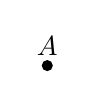
\begin{tikzpicture}
\fill (0,0) circle (2pt);
\node[above] at (0,0) {\(A\)};
\end{tikzpicture}
\end{centereddiagram}

%%%%%%%%%%%%%%%%%%%%%%%%%%%%%%%%%%%%%%%%%%%%%%%%%%%%%%%%%%%%
\subsection{Lines}
\label{subsec:euclidean-lines}
%%%%%%%%%%%%%%%%%%%%%%%%%%%%%%%%%%%%%%%%%%%%%%%%%%%%%%%%%%%%

A line extends infinitely in both directions.

The line through distinct points \(A\) and \(B\) is denoted

\[ \overleftrightarrow{AB}. \]

This is read ``line \(AB\).''

\begin{centereddiagram}
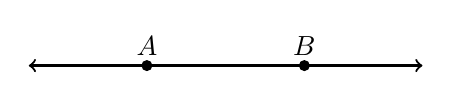
\begin{tikzpicture}
\draw[<->,thick] (-2.5,0)--(2.5,0);
\fill (-1,0) circle (2pt);
\fill (1,0) circle (2pt);
\node[above] at (-1,0) {\(A\)};
\node[above] at (1,0) {\(B\)};
\end{tikzpicture}
\end{centereddiagram}

Two distinct points determine exactly one line.

%%%%%%%%%%%%%%%%%%%%%%%%%%%%%%%%%%%%%%%%%%%%%%%%%%%%%%%%%%%%
\subsection{Line Segments}
\label{subsec:line-segments}
%%%%%%%%%%%%%%%%%%%%%%%%%%%%%%%%%%%%%%%%%%%%%%%%%%%%%%%%%%%%

The portion of a line between points \(A\) and \(B\), including both
endpoints, is the line segment

\[ \overline{AB}. \]

The notation is read ``segment \(AB\).''

Its length is usually written

\[ AB. \]

Thus

\[
\overline{AB}
\]

denotes the geometric segment, while

\[
AB
\]

often denotes its numerical length.

\begin{centereddiagram}
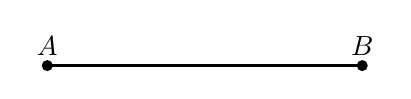
\begin{tikzpicture}
\draw[thick] (-2,0)--(2,0);
\fill (-2,0) circle (2pt);
\fill (2,0) circle (2pt);
\node[above] at (-2,0) {\(A\)};
\node[above] at (2,0) {\(B\)};
\end{tikzpicture}
\end{centereddiagram}

%%%%%%%%%%%%%%%%%%%%%%%%%%%%%%%%%%%%%%%%%%%%%%%%%%%%%%%%%%%%
\subsection{Rays}
\label{subsec:euclidean-rays}
%%%%%%%%%%%%%%%%%%%%%%%%%%%%%%%%%%%%%%%%%%%%%%%%%%%%%%%%%%%%

A ray begins at one endpoint and extends infinitely in one direction.

The ray beginning at \(A\) and passing through \(B\) is

\[ \overrightarrow{AB}. \]

This is read ``ray \(AB\).''

The order matters:

\[ \overrightarrow{AB}\neq\overrightarrow{BA} \]

in general.

\begin{centereddiagram}
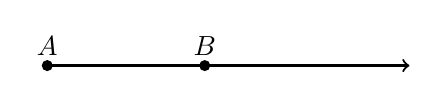
\begin{tikzpicture}
\draw[->,thick] (-2,0)--(2.6,0);
\fill (-2,0) circle (2pt);
\fill (0,0) circle (2pt);
\node[above] at (-2,0) {\(A\)};
\node[above] at (0,0) {\(B\)};
\end{tikzpicture}
\end{centereddiagram}

%%%%%%%%%%%%%%%%%%%%%%%%%%%%%%%%%%%%%%%%%%%%%%%%%%%%%%%%%%%%
\subsection{Planes}
\label{subsec:euclidean-planes}
%%%%%%%%%%%%%%%%%%%%%%%%%%%%%%%%%%%%%%%%%%%%%%%%%%%%%%%%%%%%

A plane is a flat two-dimensional surface extending infinitely in every
direction within itself.

Three noncollinear points determine exactly one plane.

\begin{centereddiagram}
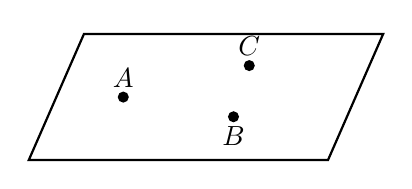
\begin{tikzpicture}
\draw[thick] (-2,-0.8)--(1.8,-0.8)--(2.5,0.8)--(-1.3,0.8)--cycle;
\fill (-0.8,0) circle (2pt);
\fill (0.6,-0.25) circle (2pt);
\fill (0.8,0.4) circle (2pt);
\node[above] at (-0.8,0) {\(A\)};
\node[below] at (0.6,-0.25) {\(B\)};
\node[above] at (0.8,0.4) {\(C\)};
\end{tikzpicture}
\end{centereddiagram}

%%%%%%%%%%%%%%%%%%%%%%%%%%%%%%%%%%%%%%%%%%%%%%%%%%%%%%%%%%%%
\subsection{Collinear and Coplanar Points}
\label{subsec:collinear-coplanar}
%%%%%%%%%%%%%%%%%%%%%%%%%%%%%%%%%%%%%%%%%%%%%%%%%%%%%%%%%%%%

\begin{definitionbox}{Collinear Points}
Points are \emph{collinear} if they lie on the same line.
\end{definitionbox}

\begin{definitionbox}{Coplanar Points}
Points or other geometric objects are \emph{coplanar} if they lie in the
same plane.
\end{definitionbox}

%%%%%%%%%%%%%%%%%%%%%%%%%%%%%%%%%%%%%%%%%%%%%%%%%%%%%%%%%%%%
\subsection{Incidence}
\label{subsec:incidence-euclidean}
%%%%%%%%%%%%%%%%%%%%%%%%%%%%%%%%%%%%%%%%%%%%%%%%%%%%%%%%%%%%

\emph{Incidence} describes which geometric objects lie on or contain other
objects.

Statements such as

\[
A\in\ell
\]

mean that point \(A\) lies on line \(\ell\).

The lowercase script-style letter \(\ell\) is commonly pronounced ``ell''
and is often used to name a line.

Incidence geometry focuses on relationships such as:

\begin{itemize}
    \item which points lie on a line;
    \item which lines pass through a point;
    \item which points and lines lie in a plane.
\end{itemize}

%%%%%%%%%%%%%%%%%%%%%%%%%%%%%%%%%%%%%%%%%%%%%%%%%%%%%%%%%%%%
\subsection{Betweenness}
\label{subsec:betweenness}
%%%%%%%%%%%%%%%%%%%%%%%%%%%%%%%%%%%%%%%%%%%%%%%%%%%%%%%%%%%%

Suppose \(A,B,C\) are distinct collinear points.

If \(B\) lies between \(A\) and \(C\), then

\[ AB+BC=AC. \]

This is the Segment Addition Postulate.

\begin{centereddiagram}
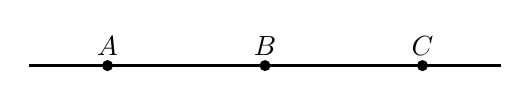
\begin{tikzpicture}
\draw[thick] (-3,0)--(3,0);
\foreach \x/\n in {-2/A,0/B,2/C}{
    \fill (\x,0) circle (2pt);
    \node[above] at (\x,0) {\(\n\)};
}
\end{tikzpicture}
\end{centereddiagram}

%%%%%%%%%%%%%%%%%%%%%%%%%%%%%%%%%%%%%%%%%%%%%%%%%%%%%%%%%%%%
\subsection{Worked Example: Segment Addition}
\label{subsec:worked-segment-addition}
%%%%%%%%%%%%%%%%%%%%%%%%%%%%%%%%%%%%%%%%%%%%%%%%%%%%%%%%%%%%

\begin{workedexamplebox}{Finding a Segment Length}

Suppose \(B\) lies between \(A\) and \(C\), with

\[ AB=7,\qquad BC=11. \]

Find \(AC\).

\begin{tabularx}{\textwidth}{@{}>{\raggedright\arraybackslash}p{0.43\textwidth}X@{}}
Use segment addition. & \(AB+BC=AC\)\\
Substitute. & \(7+11=AC\)\\
Simplify. & \(AC=18\)
\end{tabularx}

\begin{answerbox}
\[ \boxed{AC=18} \]
\end{answerbox}
\end{workedexamplebox}

%%%%%%%%%%%%%%%%%%%%%%%%%%%%%%%%%%%%%%%%%%%%%%%%%%%%%%%%%%%%
\subsection{Distance}
\label{subsec:euclidean-distance}
%%%%%%%%%%%%%%%%%%%%%%%%%%%%%%%%%%%%%%%%%%%%%%%%%%%%%%%%%%%%

Distance measures separation between points.

In classical geometry, distance satisfies several fundamental properties:

\[
AB\geq0,\qquad AB=BA.
\]

Furthermore,

\[ AB=0\iff A=B. \]

The symbol

\[ \iff \]

means ``if and only if.''

For three points, distance satisfies the Triangle Inequality:

\[ \boxed{AC\leq AB+BC.} \]

Equality occurs when the relevant points lie collinearly with \(B\) between
\(A\) and \(C\).

%%%%%%%%%%%%%%%%%%%%%%%%%%%%%%%%%%%%%%%%%%%%%%%%%%%%%%%%%%%%
\subsection{Congruent Segments}
\label{subsec:congruent-segments}
%%%%%%%%%%%%%%%%%%%%%%%%%%%%%%%%%%%%%%%%%%%%%%%%%%%%%%%%%%%%

\begin{definitionbox}{Congruent Segments}
Two line segments are \emph{congruent} if they have equal length.
\end{definitionbox}

The notation

\[ \overline{AB}\cong\overline{CD} \]

is read ``segment \(AB\) is congruent to segment \(CD\).''

It means

\[ AB=CD. \]

The symbol \(\cong\) is the congruence symbol.

%%%%%%%%%%%%%%%%%%%%%%%%%%%%%%%%%%%%%%%%%%%%%%%%%%%%%%%%%%%%
\subsection{Midpoints}
\label{subsec:midpoints-euclidean}
%%%%%%%%%%%%%%%%%%%%%%%%%%%%%%%%%%%%%%%%%%%%%%%%%%%%%%%%%%%%

\begin{definitionbox}{Midpoint}
A point \(M\) is the \emph{midpoint} of \(\overline{AB}\) if \(M\) lies on
the segment and

\[ AM=MB. \]
\end{definitionbox}

\begin{centereddiagram}
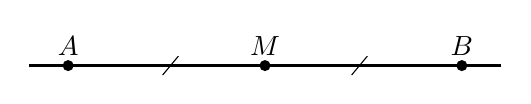
\begin{tikzpicture}
\draw[thick] (-3,0)--(3,0);
\foreach \x/\n in {-2.5/A,0/M,2.5/B}{
    \fill (\x,0) circle (2pt);
    \node[above] at (\x,0) {\(\n\)};
}
\draw (-1.3,-0.12)--(-1.1,0.12);
\draw (1.1,-0.12)--(1.3,0.12);
\end{tikzpicture}
\end{centereddiagram}

Matching tick marks indicate congruent segments.

%%%%%%%%%%%%%%%%%%%%%%%%%%%%%%%%%%%%%%%%%%%%%%%%%%%%%%%%%%%%
\subsection{Angles}
\label{subsec:euclidean-angles}
%%%%%%%%%%%%%%%%%%%%%%%%%%%%%%%%%%%%%%%%%%%%%%%%%%%%%%%%%%%%

\begin{definitionbox}{Angle}
An \emph{angle} is formed by two rays having a common endpoint.
\end{definitionbox}

The common endpoint is called the \emph{vertex}.

If rays

\[ \overrightarrow{BA}\qquad\text{and}\qquad\overrightarrow{BC} \]

share vertex \(B\), the angle is written

\[ \angle ABC. \]

The middle letter identifies the vertex.

%%%%%%%%%%%%%%%%%%%%%%%%%%%%%%%%%%%%%%%%%%%%%%%%%%%%%%%%%%%%
\subsection{Angle Visual}
\label{subsec:angle-visual}
%%%%%%%%%%%%%%%%%%%%%%%%%%%%%%%%%%%%%%%%%%%%%%%%%%%%%%%%%%%%

\begin{centereddiagram}
\begin{tikzpicture}
\draw[->,thick] (0,0)--(3,0);
\draw[->,thick] (0,0)--(2,1.8);
\fill (0,0) circle (2pt);
\node[below left] at (0,0) {\(B\)};
\node[right] at (3,0) {\(C\)};
\node[above right] at (2,1.8) {\(A\)};
\draw (0.8,0) arc[start angle=0,end angle=42,radius=0.8];
\end{tikzpicture}
\end{centereddiagram}

The angle may also be denoted

\[ \angle B \]

when there is no ambiguity.

%%%%%%%%%%%%%%%%%%%%%%%%%%%%%%%%%%%%%%%%%%%%%%%%%%%%%%%%%%%%
\subsection{Angle Measure}
\label{subsec:angle-measure}
%%%%%%%%%%%%%%%%%%%%%%%%%%%%%%%%%%%%%%%%%%%%%%%%%%%%%%%%%%%%

The measure of an angle \(\angle ABC\) is written

\[ m\angle ABC. \]

The symbol \(m\) means ``measure of.''

In elementary Euclidean geometry, angle measure is commonly expressed in
degrees.

A full rotation contains

\[ 360^\circ. \]

A half rotation contains

\[ 180^\circ, \]

and a quarter rotation contains

\[ 90^\circ. \]

%%%%%%%%%%%%%%%%%%%%%%%%%%%%%%%%%%%%%%%%%%%%%%%%%%%%%%%%%%%%
\subsection{Classification of Angles}
\label{subsec:classification-angles}
%%%%%%%%%%%%%%%%%%%%%%%%%%%%%%%%%%%%%%%%%%%%%%%%%%%%%%%%%%%%

Angles are classified by measure:

\[
\begin{array}{c|c}
\textbf{Type} & \textbf{Measure}\\
\hline
\text{acute} & 0^\circ<\theta<90^\circ\\
\text{right} & \theta=90^\circ\\
\text{obtuse} & 90^\circ<\theta<180^\circ\\
\text{straight} & \theta=180^\circ\\
\text{reflex} & 180^\circ<\theta<360^\circ
\end{array}
\]

The Greek letter

\[ \theta \]

is \emph{theta}, pronounced ``THAY-tuh'' or ``THEE-tuh,'' and commonly
represents an angle.

%%%%%%%%%%%%%%%%%%%%%%%%%%%%%%%%%%%%%%%%%%%%%%%%%%%%%%%%%%%%
\subsection{Angle Classification Visual}
\label{subsec:angle-classification-visual}
%%%%%%%%%%%%%%%%%%%%%%%%%%%%%%%%%%%%%%%%%%%%%%%%%%%%%%%%%%%%

\begin{centereddiagram}
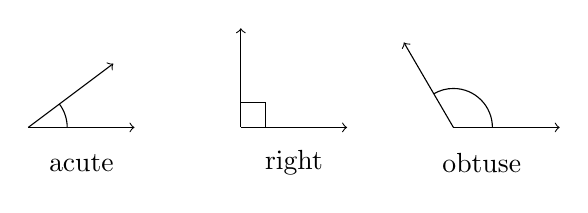
\begin{tikzpicture}[scale=0.9]
% acute
\draw[->] (0,0)--(1.5,0);
\draw[->] (0,0)--(1.2,0.9);
\draw (0.55,0) arc[start angle=0,end angle=37,radius=.55];
\node at (.75,-.5) {acute};

% right
\begin{scope}[xshift=3cm]
\draw[->] (0,0)--(1.5,0);
\draw[->] (0,0)--(0,1.4);
\draw (0.35,0)--(0.35,0.35)--(0,0.35);
\node at (.75,-.5) {right};
\end{scope}

% obtuse
\begin{scope}[xshift=6cm]
\draw[->] (0,0)--(1.5,0);
\draw[->] (0,0)--(-.7,1.2);
\draw (.55,0) arc[start angle=0,end angle=120,radius=.55];
\node at (.4,-.5) {obtuse};
\end{scope}
\end{tikzpicture}
\end{centereddiagram}

%%%%%%%%%%%%%%%%%%%%%%%%%%%%%%%%%%%%%%%%%%%%%%%%%%%%%%%%%%%%
\subsection{Congruent Angles}
\label{subsec:congruent-angles}
%%%%%%%%%%%%%%%%%%%%%%%%%%%%%%%%%%%%%%%%%%%%%%%%%%%%%%%%%%%%

Two angles are congruent when they have equal measure.

Thus

\[ \angle ABC\cong\angle DEF \]

means

\[ m\angle ABC=m\angle DEF. \]

%%%%%%%%%%%%%%%%%%%%%%%%%%%%%%%%%%%%%%%%%%%%%%%%%%%%%%%%%%%%
\subsection{Angle Addition}
\label{subsec:angle-addition}
%%%%%%%%%%%%%%%%%%%%%%%%%%%%%%%%%%%%%%%%%%%%%%%%%%%%%%%%%%%%

If ray \(\overrightarrow{BD}\) lies inside \(\angle ABC\), then

\[ \boxed{m\angle ABD+m\angle DBC=m\angle ABC.} \]

This is the Angle Addition Postulate.

%%%%%%%%%%%%%%%%%%%%%%%%%%%%%%%%%%%%%%%%%%%%%%%%%%%%%%%%%%%%
\subsection{Angle Bisectors}
\label{subsec:angle-bisectors}
%%%%%%%%%%%%%%%%%%%%%%%%%%%%%%%%%%%%%%%%%%%%%%%%%%%%%%%%%%%%

\begin{definitionbox}{Angle Bisector}
An \emph{angle bisector} is a ray that divides an angle into two congruent
angles.
\end{definitionbox}

If \(\overrightarrow{BD}\) bisects \(\angle ABC\), then

\[ m\angle ABD=m\angle DBC. \]

%%%%%%%%%%%%%%%%%%%%%%%%%%%%%%%%%%%%%%%%%%%%%%%%%%%%%%%%%%%%
\subsection{Complementary and Supplementary Angles}
\label{subsec:complementary-supplementary}
%%%%%%%%%%%%%%%%%%%%%%%%%%%%%%%%%%%%%%%%%%%%%%%%%%%%%%%%%%%%

\begin{definitionbox}{Complementary Angles}
Two angles are \emph{complementary} if their measures sum to

\[ 90^\circ. \]
\end{definitionbox}

\begin{definitionbox}{Supplementary Angles}
Two angles are \emph{supplementary} if their measures sum to

\[ 180^\circ. \]
\end{definitionbox}

Thus

\[ \alpha+\beta=90^\circ \]

describes complementary angle measures, while

\[ \alpha+\beta=180^\circ \]

describes supplementary angle measures.

The Greek letter \(\alpha\) is \emph{alpha}, and \(\beta\) is \emph{beta}.

%%%%%%%%%%%%%%%%%%%%%%%%%%%%%%%%%%%%%%%%%%%%%%%%%%%%%%%%%%%%
\subsection{Linear Pairs}
\label{subsec:linear-pairs}
%%%%%%%%%%%%%%%%%%%%%%%%%%%%%%%%%%%%%%%%%%%%%%%%%%%%%%%%%%%%

Two adjacent angles form a \emph{linear pair} when their noncommon sides are
opposite rays.

Their measures sum to

\[ \boxed{180^\circ.} \]

Therefore every linear pair consists of supplementary angles.

%%%%%%%%%%%%%%%%%%%%%%%%%%%%%%%%%%%%%%%%%%%%%%%%%%%%%%%%%%%%
\subsection{Vertical Angles}
\label{subsec:vertical-angles}
%%%%%%%%%%%%%%%%%%%%%%%%%%%%%%%%%%%%%%%%%%%%%%%%%%%%%%%%%%%%

When two lines intersect, opposite angles are called \emph{vertical angles}.

\begin{centereddiagram}
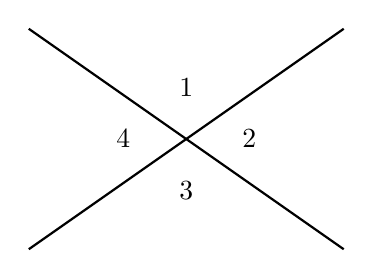
\begin{tikzpicture}
\draw[thick] (-2,-1.4)--(2,1.4);
\draw[thick] (-2,1.4)--(2,-1.4);
\node at (0,0.65) {\(1\)};
\node at (0.8,0) {\(2\)};
\node at (0,-0.65) {\(3\)};
\node at (-0.8,0) {\(4\)};
\end{tikzpicture}
\end{centereddiagram}

The Vertical Angles Theorem states

\[ \boxed{\angle1\cong\angle3,\qquad\angle2\cong\angle4.} \]

%%%%%%%%%%%%%%%%%%%%%%%%%%%%%%%%%%%%%%%%%%%%%%%%%%%%%%%%%%%%
\subsection{Worked Example: Vertical Angles}
\label{subsec:worked-vertical-angles}
%%%%%%%%%%%%%%%%%%%%%%%%%%%%%%%%%%%%%%%%%%%%%%%%%%%%%%%%%%%%

\begin{workedexamplebox}{Solving for a Vertical Angle}

Suppose two vertical angles have measures

\[ 5x+10^\circ\qquad\text{and}\qquad8x-35^\circ. \]

\begin{tabularx}{\textwidth}{@{}>{\raggedright\arraybackslash}p{0.43\textwidth}X@{}}
Vertical angles are congruent. & \(5x+10=8x-35\)\\
Move the \(x\)-terms. & \(45=3x\)\\
Solve. & \(x=15\)\\
Find the angle. & \(5(15)+10=85^\circ\)
\end{tabularx}

\begin{answerbox}
\[ \boxed{x=15,\qquad m\angle=85^\circ} \]
\end{answerbox}
\end{workedexamplebox}

%%%%%%%%%%%%%%%%%%%%%%%%%%%%%%%%%%%%%%%%%%%%%%%%%%%%%%%%%%%%
\subsection{Perpendicular Lines}
\label{subsec:perpendicular-lines-euclidean}
%%%%%%%%%%%%%%%%%%%%%%%%%%%%%%%%%%%%%%%%%%%%%%%%%%%%%%%%%%%%

\begin{definitionbox}{Perpendicular Lines}
Two lines are \emph{perpendicular} if they intersect to form right angles.
\end{definitionbox}

The notation

\[ \ell\perp m \]

is read ``line \(\ell\) is perpendicular to line \(m\).''

%%%%%%%%%%%%%%%%%%%%%%%%%%%%%%%%%%%%%%%%%%%%%%%%%%%%%%%%%%%%
\subsection{Parallel Lines}
\label{subsec:parallel-lines-euclidean}
%%%%%%%%%%%%%%%%%%%%%%%%%%%%%%%%%%%%%%%%%%%%%%%%%%%%%%%%%%%%

\begin{definitionbox}{Parallel Lines}
Two distinct coplanar lines are \emph{parallel} if they do not intersect.
\end{definitionbox}

The notation

\[ \ell\parallel m \]

is read ``line \(\ell\) is parallel to line \(m\).''

%%%%%%%%%%%%%%%%%%%%%%%%%%%%%%%%%%%%%%%%%%%%%%%%%%%%%%%%%%%%
\subsection{Euclid's Parallel Postulate}
\label{subsec:euclid-parallel-postulate}
%%%%%%%%%%%%%%%%%%%%%%%%%%%%%%%%%%%%%%%%%%%%%%%%%%%%%%%%%%%%

One modern equivalent of Euclid's parallel postulate is:

\begin{importantbox}
Given a line \(\ell\) and a point \(P\) not on \(\ell\), there exists exactly
one line through \(P\) parallel to \(\ell\).
\end{importantbox}

This property distinguishes Euclidean geometry from major non-Euclidean
geometries.

Changing the parallel postulate produces fundamentally different geometric
systems.

%%%%%%%%%%%%%%%%%%%%%%%%%%%%%%%%%%%%%%%%%%%%%%%%%%%%%%%%%%%%
\subsection{Transversals}
\label{subsec:transversals}
%%%%%%%%%%%%%%%%%%%%%%%%%%%%%%%%%%%%%%%%%%%%%%%%%%%%%%%%%%%%

A \emph{transversal} is a line intersecting two or more coplanar lines at
distinct points.

When a transversal intersects parallel lines, several angle relationships
appear.

\begin{centereddiagram}
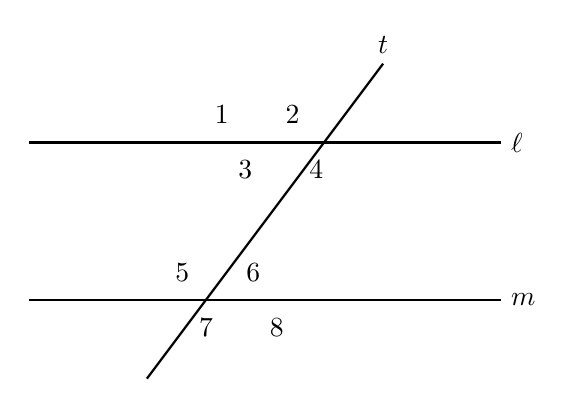
\begin{tikzpicture}
\draw[thick] (-3,1)--(3,1);
\draw[thick] (-3,-1)--(3,-1);
\draw[thick] (-1.5,-2)--(1.5,2);

\node[right] at (3,1) {\(\ell\)};
\node[right] at (3,-1) {\(m\)};
\node[above] at (1.5,2) {\(t\)};

\node at (-0.55,1.35) {\(1\)};
\node at (0.35,1.35) {\(2\)};
\node at (-0.25,0.65) {\(3\)};
\node at (0.65,0.65) {\(4\)};

\node at (-1.05,-0.65) {\(5\)};
\node at (-0.15,-0.65) {\(6\)};
\node at (-0.75,-1.35) {\(7\)};
\node at (0.15,-1.35) {\(8\)};
\end{tikzpicture}
\end{centereddiagram}

Assume

\[ \ell\parallel m. \]

%%%%%%%%%%%%%%%%%%%%%%%%%%%%%%%%%%%%%%%%%%%%%%%%%%%%%%%%%%%%
\subsection{Corresponding Angles}
\label{subsec:corresponding-angles}
%%%%%%%%%%%%%%%%%%%%%%%%%%%%%%%%%%%%%%%%%%%%%%%%%%%%%%%%%%%%

Corresponding angles occupy matching positions at the two intersections.

For parallel lines,

\[ \boxed{\text{corresponding angles are congruent}.} \]

For example,

\[ \angle1\cong\angle5. \]

%%%%%%%%%%%%%%%%%%%%%%%%%%%%%%%%%%%%%%%%%%%%%%%%%%%%%%%%%%%%
\subsection{Alternate Interior Angles}
\label{subsec:alternate-interior-angles}
%%%%%%%%%%%%%%%%%%%%%%%%%%%%%%%%%%%%%%%%%%%%%%%%%%%%%%%%%%%%

Alternate interior angles lie between the parallel lines on opposite sides
of the transversal.

For parallel lines,

\[ \boxed{\text{alternate interior angles are congruent}.} \]

%%%%%%%%%%%%%%%%%%%%%%%%%%%%%%%%%%%%%%%%%%%%%%%%%%%%%%%%%%%%
\subsection{Alternate Exterior Angles}
\label{subsec:alternate-exterior-angles}
%%%%%%%%%%%%%%%%%%%%%%%%%%%%%%%%%%%%%%%%%%%%%%%%%%%%%%%%%%%%

Alternate exterior angles lie outside the parallel lines on opposite sides
of the transversal.

For parallel lines,

\[ \boxed{\text{alternate exterior angles are congruent}.} \]

%%%%%%%%%%%%%%%%%%%%%%%%%%%%%%%%%%%%%%%%%%%%%%%%%%%%%%%%%%%%
\subsection{Same-Side Interior Angles}
\label{subsec:same-side-interior}
%%%%%%%%%%%%%%%%%%%%%%%%%%%%%%%%%%%%%%%%%%%%%%%%%%%%%%%%%%%%

Same-side interior angles lie between the parallel lines on the same side of
the transversal.

Their measures satisfy

\[ \boxed{\alpha+\beta=180^\circ.} \]

They are therefore supplementary.

%%%%%%%%%%%%%%%%%%%%%%%%%%%%%%%%%%%%%%%%%%%%%%%%%%%%%%%%%%%%
\subsection{Triangles}
\label{subsec:euclidean-triangles}
%%%%%%%%%%%%%%%%%%%%%%%%%%%%%%%%%%%%%%%%%%%%%%%%%%%%%%%%%%%%

\begin{definitionbox}{Triangle}
A \emph{triangle} is a polygon formed by three noncollinear points connected
by three line segments.
\end{definitionbox}

The triangle with vertices \(A,B,C\) is denoted

\[ \triangle ABC. \]

The symbol \(\triangle\) is read ``triangle.''

\begin{centereddiagram}
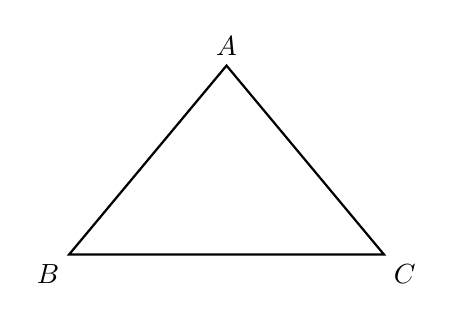
\begin{tikzpicture}
\coordinate (A) at (0,2.4);
\coordinate (B) at (-2,0);
\coordinate (C) at (2,0);
\draw[thick] (A)--(B)--(C)--cycle;
\node[above] at (A) {\(A\)};
\node[below left] at (B) {\(B\)};
\node[below right] at (C) {\(C\)};
\end{tikzpicture}
\end{centereddiagram}

%%%%%%%%%%%%%%%%%%%%%%%%%%%%%%%%%%%%%%%%%%%%%%%%%%%%%%%%%%%%
\subsection{Classification by Side Length}
\label{subsec:triangle-classification-sides}
%%%%%%%%%%%%%%%%%%%%%%%%%%%%%%%%%%%%%%%%%%%%%%%%%%%%%%%%%%%%

Triangles can be classified by their side lengths.

\[
\begin{array}{c|c}
\textbf{Triangle} & \textbf{Side relationship}\\
\hline
\text{scalene} & \text{no congruent sides}\\
\text{isosceles} & \text{at least two congruent sides}\\
\text{equilateral} & \text{three congruent sides}
\end{array}
\]

An equilateral triangle is therefore a special type of isosceles triangle
under the inclusive definition.

%%%%%%%%%%%%%%%%%%%%%%%%%%%%%%%%%%%%%%%%%%%%%%%%%%%%%%%%%%%%
\subsection{Classification by Angle}
\label{subsec:triangle-classification-angles}
%%%%%%%%%%%%%%%%%%%%%%%%%%%%%%%%%%%%%%%%%%%%%%%%%%%%%%%%%%%%

Triangles can also be classified by their angles:

\[
\begin{array}{c|c}
\textbf{Triangle} & \textbf{Angle condition}\\
\hline
\text{acute} & \text{all three angles acute}\\
\text{right} & \text{one right angle}\\
\text{obtuse} & \text{one obtuse angle}\\
\text{equiangular} & \text{three congruent angles}
\end{array}
\]

%%%%%%%%%%%%%%%%%%%%%%%%%%%%%%%%%%%%%%%%%%%%%%%%%%%%%%%%%%%%
\subsection{Triangle Sum Theorem}
\label{subsec:triangle-sum-theorem}
%%%%%%%%%%%%%%%%%%%%%%%%%%%%%%%%%%%%%%%%%%%%%%%%%%%%%%%%%%%%

\begin{theorem}[Triangle Sum Theorem]
The interior angles of a Euclidean triangle have total measure

\[ \boxed{180^\circ.} \]
\end{theorem}

Thus if the angles have measures \(\alpha,\beta,\gamma\), then

\[ \boxed{\alpha+\beta+\gamma=180^\circ.} \]

The Greek letter \(\gamma\) is \emph{gamma}, pronounced ``GAM-uh.''

%%%%%%%%%%%%%%%%%%%%%%%%%%%%%%%%%%%%%%%%%%%%%%%%%%%%%%%%%%%%
\subsection{Visual Proof of the Triangle Sum}
\label{subsec:triangle-sum-visual}
%%%%%%%%%%%%%%%%%%%%%%%%%%%%%%%%%%%%%%%%%%%%%%%%%%%%%%%%%%%%

\begin{centereddiagram}
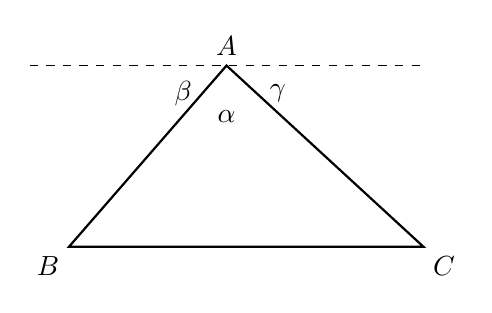
\begin{tikzpicture}
\coordinate (A) at (0,2.3);
\coordinate (B) at (-2,0);
\coordinate (C) at (2.5,0);

\draw[thick] (A)--(B)--(C)--cycle;
\draw[dashed] (-2.5,2.3)--(2.5,2.3);

\node[above] at (A) {\(A\)};
\node[below left] at (B) {\(B\)};
\node[below right] at (C) {\(C\)};

\node at (-0.55,1.95) {\(\beta\)};
\node at (0,1.65) {\(\alpha\)};
\node at (0.65,1.95) {\(\gamma\)};
\end{tikzpicture}
\end{centereddiagram}

Draw a line through \(A\) parallel to \(\overline{BC}\).

Alternate interior angles reproduce the angles at \(B\) and \(C\) along the
line through \(A\).

Together with the angle at \(A\), they form a straight angle.

Therefore

\[ \alpha+\beta+\gamma=180^\circ. \]

%%%%%%%%%%%%%%%%%%%%%%%%%%%%%%%%%%%%%%%%%%%%%%%%%%%%%%%%%%%%
\subsection{Worked Example: Triangle Angles}
\label{subsec:worked-triangle-angles}
%%%%%%%%%%%%%%%%%%%%%%%%%%%%%%%%%%%%%%%%%%%%%%%%%%%%%%%%%%%%

\begin{workedexamplebox}{Finding the Third Angle}

A triangle has angles

\[ 47^\circ,\qquad68^\circ,\qquad x. \]

\begin{tabularx}{\textwidth}{@{}>{\raggedright\arraybackslash}p{0.43\textwidth}X@{}}
Use the Triangle Sum Theorem. & \(47+68+x=180\)\\
Combine known angles. & \(115+x=180\)\\
Solve. & \(x=65\)
\end{tabularx}

\begin{answerbox}
\[ \boxed{x=65^\circ} \]
\end{answerbox}
\end{workedexamplebox}

%%%%%%%%%%%%%%%%%%%%%%%%%%%%%%%%%%%%%%%%%%%%%%%%%%%%%%%%%%%%
\subsection{Exterior Angles of Triangles}
\label{subsec:triangle-exterior-angle}
%%%%%%%%%%%%%%%%%%%%%%%%%%%%%%%%%%%%%%%%%%%%%%%%%%%%%%%%%%%%

An exterior angle is formed by extending one side of a triangle.

\begin{theorem}[Exterior Angle Theorem]
The measure of an exterior angle of a triangle equals the sum of the two
nonadjacent interior angles.
\end{theorem}

Thus

\[ \boxed{\theta=\alpha+\beta.} \]

%%%%%%%%%%%%%%%%%%%%%%%%%%%%%%%%%%%%%%%%%%%%%%%%%%%%%%%%%%%%
\subsection{Isosceles Triangle Theorem}
\label{subsec:isosceles-triangle-theorem}
%%%%%%%%%%%%%%%%%%%%%%%%%%%%%%%%%%%%%%%%%%%%%%%%%%%%%%%%%%%%

\begin{theorem}[Isosceles Triangle Theorem]
If two sides of a triangle are congruent, then the angles opposite those
sides are congruent.
\end{theorem}

Thus if

\[ AB=AC, \]

then

\[ \angle B\cong\angle C. \]

The converse is also true.

%%%%%%%%%%%%%%%%%%%%%%%%%%%%%%%%%%%%%%%%%%%%%%%%%%%%%%%%%%%%
\subsection{Equilateral Triangles}
\label{subsec:equilateral-triangles}
%%%%%%%%%%%%%%%%%%%%%%%%%%%%%%%%%%%%%%%%%%%%%%%%%%%%%%%%%%%%

If all three sides are congruent, all three angles are congruent.

Since their sum is \(180^\circ\),

\[ 3\theta=180^\circ. \]

Therefore

\[ \boxed{\theta=60^\circ.} \]

Every equilateral triangle is equiangular, and every equiangular Euclidean
triangle is equilateral.

%%%%%%%%%%%%%%%%%%%%%%%%%%%%%%%%%%%%%%%%%%%%%%%%%%%%%%%%%%%%
\subsection{Triangle Inequality}
\label{subsec:triangle-inequality-geometry}
%%%%%%%%%%%%%%%%%%%%%%%%%%%%%%%%%%%%%%%%%%%%%%%%%%%%%%%%%%%%

\begin{theorem}[Triangle Inequality]
For any triangle with side lengths \(a,b,c\),

\[ \boxed{a+b>c,\qquad a+c>b,\qquad b+c>a.} \]
\end{theorem}

The sum of the lengths of any two sides must exceed the length of the third.

%%%%%%%%%%%%%%%%%%%%%%%%%%%%%%%%%%%%%%%%%%%%%%%%%%%%%%%%%%%%
\subsection{Worked Example: Can These Form a Triangle?}
\label{subsec:worked-triangle-inequality}
%%%%%%%%%%%%%%%%%%%%%%%%%%%%%%%%%%%%%%%%%%%%%%%%%%%%%%%%%%%%

\begin{workedexamplebox}{Testing Side Lengths}

Can side lengths

\[ 4,\qquad7,\qquad12 \]

form a triangle?

\begin{tabularx}{\textwidth}{@{}>{\raggedright\arraybackslash}p{0.43\textwidth}X@{}}
Check the two shorter sides. & \(4+7=11\)\\
Compare with the longest side. & \(11<12\)\\
Apply the Triangle Inequality. & The required inequality fails.
\end{tabularx}

\begin{answerbox}
\[ \boxed{\text{No triangle exists with side lengths }4,7,12.} \]
\end{answerbox}
\end{workedexamplebox}

%%%%%%%%%%%%%%%%%%%%%%%%%%%%%%%%%%%%%%%%%%%%%%%%%%%%%%%%%%%%
\subsection{Triangle Congruence}
\label{subsec:triangle-congruence}
%%%%%%%%%%%%%%%%%%%%%%%%%%%%%%%%%%%%%%%%%%%%%%%%%%%%%%%%%%%%

Two triangles are congruent when they have the same size and shape.

The notation

\[ \triangle ABC\cong\triangle DEF \]

indicates the correspondence

\[ A\leftrightarrow D,\qquad B\leftrightarrow E,\qquad C\leftrightarrow F. \]

Therefore corresponding sides and angles are congruent.

%%%%%%%%%%%%%%%%%%%%%%%%%%%%%%%%%%%%%%%%%%%%%%%%%%%%%%%%%%%%
\subsection{SSS Congruence}
\label{subsec:sss-congruence}
%%%%%%%%%%%%%%%%%%%%%%%%%%%%%%%%%%%%%%%%%%%%%%%%%%%%%%%%%%%%

\begin{theorem}[Side--Side--Side Congruence]
If three sides of one triangle are congruent to the three corresponding
sides of another triangle, then the triangles are congruent.
\end{theorem}

This criterion is abbreviated

\[ \boxed{\mathrm{SSS}.} \]

%%%%%%%%%%%%%%%%%%%%%%%%%%%%%%%%%%%%%%%%%%%%%%%%%%%%%%%%%%%%
\subsection{SAS Congruence}
\label{subsec:sas-congruence}
%%%%%%%%%%%%%%%%%%%%%%%%%%%%%%%%%%%%%%%%%%%%%%%%%%%%%%%%%%%%

\begin{theorem}[Side--Angle--Side Congruence]
If two sides and the included angle of one triangle are congruent to the
corresponding parts of another triangle, then the triangles are congruent.
\end{theorem}

This is abbreviated

\[ \boxed{\mathrm{SAS}.} \]

The word \emph{included} is essential.

%%%%%%%%%%%%%%%%%%%%%%%%%%%%%%%%%%%%%%%%%%%%%%%%%%%%%%%%%%%%
\subsection{ASA and AAS Congruence}
\label{subsec:asa-aas-congruence}
%%%%%%%%%%%%%%%%%%%%%%%%%%%%%%%%%%%%%%%%%%%%%%%%%%%%%%%%%%%%

Two additional criteria are:

\[
\boxed{\mathrm{ASA}}
\]

for Angle--Side--Angle, and

\[
\boxed{\mathrm{AAS}}
\]

for Angle--Angle--Side.

Both determine a triangle uniquely up to congruence.

%%%%%%%%%%%%%%%%%%%%%%%%%%%%%%%%%%%%%%%%%%%%%%%%%%%%%%%%%%%%
\subsection{HL Congruence}
\label{subsec:hl-congruence}
%%%%%%%%%%%%%%%%%%%%%%%%%%%%%%%%%%%%%%%%%%%%%%%%%%%%%%%%%%%%

For right triangles, one can use the Hypotenuse--Leg criterion.

\begin{theorem}[Hypotenuse--Leg Congruence]
If the hypotenuse and one corresponding leg of two right triangles are
congruent, then the triangles are congruent.
\end{theorem}

This is abbreviated

\[ \boxed{\mathrm{HL}.} \]

%%%%%%%%%%%%%%%%%%%%%%%%%%%%%%%%%%%%%%%%%%%%%%%%%%%%%%%%%%%%
\subsection{Why SSA Is Not a General Congruence Criterion}
\label{subsec:ssa-ambiguous}
%%%%%%%%%%%%%%%%%%%%%%%%%%%%%%%%%%%%%%%%%%%%%%%%%%%%%%%%%%%%

Side--Side--Angle information does not generally determine a unique
triangle.

Different triangles can satisfy the same two side lengths and a
nonincluded angle.

This is known as the \emph{ambiguous case}.

\begin{warningbox}
SSA is not a general triangle congruence theorem.

Do not confuse SSA with SAS.
\end{warningbox}

%%%%%%%%%%%%%%%%%%%%%%%%%%%%%%%%%%%%%%%%%%%%%%%%%%%%%%%%%%%%
\subsection{CPCTC}
\label{subsec:cpctc}
%%%%%%%%%%%%%%%%%%%%%%%%%%%%%%%%%%%%%%%%%%%%%%%%%%%%%%%%%%%%

Once two triangles have been proven congruent, all corresponding parts are
congruent.

This principle is often abbreviated \emph{CPCTC}:

\begin{center}
Corresponding Parts of Congruent Triangles are Congruent.
\end{center}

Congruence criteria establish triangle congruence; CPCTC is then used to
deduce additional corresponding relationships.

%%%%%%%%%%%%%%%%%%%%%%%%%%%%%%%%%%%%%%%%%%%%%%%%%%%%%%%%%%%%
\subsection{Triangle Similarity}
\label{subsec:triangle-similarity}
%%%%%%%%%%%%%%%%%%%%%%%%%%%%%%%%%%%%%%%%%%%%%%%%%%%%%%%%%%%%

Two triangles are similar when they have the same shape but not necessarily
the same size.

The notation

\[ \triangle ABC\sim\triangle DEF \]

is read ``triangle \(ABC\) is similar to triangle \(DEF\).''

The symbol \(\sim\) here denotes geometric similarity.

Corresponding angles are congruent and corresponding side lengths are
proportional.

%%%%%%%%%%%%%%%%%%%%%%%%%%%%%%%%%%%%%%%%%%%%%%%%%%%%%%%%%%%%
\subsection{AA Similarity}
\label{subsec:aa-similarity}
%%%%%%%%%%%%%%%%%%%%%%%%%%%%%%%%%%%%%%%%%%%%%%%%%%%%%%%%%%%%

\begin{theorem}[Angle--Angle Similarity]
If two angles of one triangle are congruent to two angles of another
triangle, then the triangles are similar.
\end{theorem}

This criterion is abbreviated

\[ \boxed{\mathrm{AA}.} \]

The third pair of angles must then also be congruent by the Triangle Sum
Theorem.

%%%%%%%%%%%%%%%%%%%%%%%%%%%%%%%%%%%%%%%%%%%%%%%%%%%%%%%%%%%%
\subsection{SAS and SSS Similarity}
\label{subsec:sas-sss-similarity}
%%%%%%%%%%%%%%%%%%%%%%%%%%%%%%%%%%%%%%%%%%%%%%%%%%%%%%%%%%%%

Triangles are also similar if:

\begin{itemize}
    \item two pairs of corresponding sides are proportional and their
    included angles are congruent --- SAS similarity;
    \item all three pairs of corresponding sides are proportional ---
    SSS similarity.
\end{itemize}

%%%%%%%%%%%%%%%%%%%%%%%%%%%%%%%%%%%%%%%%%%%%%%%%%%%%%%%%%%%%
\subsection{Scale Factor}
\label{subsec:scale-factor-similarity}
%%%%%%%%%%%%%%%%%%%%%%%%%%%%%%%%%%%%%%%%%%%%%%%%%%%%%%%%%%%%

Suppose

\[ \triangle ABC\sim\triangle DEF. \]

Then corresponding side ratios are equal:

\[ \boxed{\frac{AB}{DE}=\frac{BC}{EF}=\frac{AC}{DF}.} \]

This common ratio determines the scale factor between the triangles.

%%%%%%%%%%%%%%%%%%%%%%%%%%%%%%%%%%%%%%%%%%%%%%%%%%%%%%%%%%%%
\subsection{Worked Example: Similar Triangles}
\label{subsec:worked-similar-triangles}
%%%%%%%%%%%%%%%%%%%%%%%%%%%%%%%%%%%%%%%%%%%%%%%%%%%%%%%%%%%%

\begin{workedexamplebox}{Finding a Missing Side}

Suppose two similar triangles have corresponding sides

\[ 6\leftrightarrow9,\qquad10\leftrightarrow x. \]

\begin{tabularx}{\textwidth}{@{}>{\raggedright\arraybackslash}p{0.43\textwidth}X@{}}
Set corresponding ratios equal. & \(\frac69=\frac{10}{x}\)\\
Cross multiply. & \(6x=90\)\\
Solve. & \(x=15\)
\end{tabularx}

\begin{answerbox}
\[ \boxed{x=15} \]
\end{answerbox}
\end{workedexamplebox}

%%%%%%%%%%%%%%%%%%%%%%%%%%%%%%%%%%%%%%%%%%%%%%%%%%%%%%%%%%%%
\subsection{Right Triangles}
\label{subsec:right-triangles-euclidean}
%%%%%%%%%%%%%%%%%%%%%%%%%%%%%%%%%%%%%%%%%%%%%%%%%%%%%%%%%%%%

A right triangle contains one \(90^\circ\) angle.

The side opposite the right angle is the \emph{hypotenuse}.

The remaining sides are the \emph{legs}.

\begin{centereddiagram}
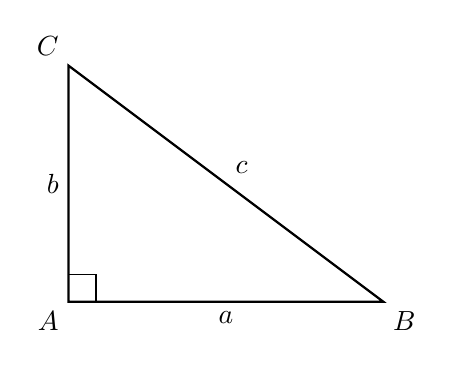
\begin{tikzpicture}
\coordinate (A) at (0,0);
\coordinate (B) at (4,0);
\coordinate (C) at (0,3);

\draw[thick] (A)--(B)--(C)--cycle;
\draw (0.35,0)--(0.35,0.35)--(0,0.35);

\node[below left] at (A) {\(A\)};
\node[below right] at (B) {\(B\)};
\node[above left] at (C) {\(C\)};

\node[below] at (2,0) {\(a\)};
\node[left] at (0,1.5) {\(b\)};
\node[above right] at (2,1.5) {\(c\)};
\end{tikzpicture}
\end{centereddiagram}

%%%%%%%%%%%%%%%%%%%%%%%%%%%%%%%%%%%%%%%%%%%%%%%%%%%%%%%%%%%%
\subsection{Pythagorean Theorem}
\label{subsec:pythagorean-theorem}
%%%%%%%%%%%%%%%%%%%%%%%%%%%%%%%%%%%%%%%%%%%%%%%%%%%%%%%%%%%%

\begin{theorem}[Pythagorean Theorem]
For a right triangle with legs \(a,b\) and hypotenuse \(c\),

\[ \boxed{a^2+b^2=c^2.} \]
\end{theorem}

This is one of the fundamental relationships of Euclidean geometry.

%%%%%%%%%%%%%%%%%%%%%%%%%%%%%%%%%%%%%%%%%%%%%%%%%%%%%%%%%%%%
\subsection{Pythagorean Area Interpretation}
\label{subsec:pythagorean-area-interpretation}
%%%%%%%%%%%%%%%%%%%%%%%%%%%%%%%%%%%%%%%%%%%%%%%%%%%%%%%%%%%%

The theorem can be interpreted geometrically:

\[
\boxed{
\text{area of square on leg }a
+
\text{area of square on leg }b
=
\text{area of square on hypotenuse }c.
}
\]

Thus the equation

\[ a^2+b^2=c^2 \]

is fundamentally an area statement.

%%%%%%%%%%%%%%%%%%%%%%%%%%%%%%%%%%%%%%%%%%%%%%%%%%%%%%%%%%%%
\subsection{Worked Example: Pythagorean Theorem}
\label{subsec:worked-pythagorean}
%%%%%%%%%%%%%%%%%%%%%%%%%%%%%%%%%%%%%%%%%%%%%%%%%%%%%%%%%%%%

\begin{workedexamplebox}{Finding the Hypotenuse}

A right triangle has legs

\[ a=6,\qquad b=8. \]

\begin{tabularx}{\textwidth}{@{}>{\raggedright\arraybackslash}p{0.43\textwidth}X@{}}
Use the Pythagorean Theorem. & \(6^2+8^2=c^2\)\\
Square. & \(36+64=c^2\)\\
Combine. & \(100=c^2\)\\
Take the positive square root. & \(c=10\)
\end{tabularx}

\begin{answerbox}
\[ \boxed{c=10} \]
\end{answerbox}
\end{workedexamplebox}

%%%%%%%%%%%%%%%%%%%%%%%%%%%%%%%%%%%%%%%%%%%%%%%%%%%%%%%%%%%%
\subsection{Converse of the Pythagorean Theorem}
\label{subsec:converse-pythagorean}
%%%%%%%%%%%%%%%%%%%%%%%%%%%%%%%%%%%%%%%%%%%%%%%%%%%%%%%%%%%%

\begin{theorem}[Converse of the Pythagorean Theorem]
If the side lengths of a triangle satisfy

\[ a^2+b^2=c^2 \]

with \(c\) the longest side, then the triangle is a right triangle.
\end{theorem}

Thus the Pythagorean relationship can be used both to compute lengths and to
classify triangles.

%%%%%%%%%%%%%%%%%%%%%%%%%%%%%%%%%%%%%%%%%%%%%%%%%%%%%%%%%%%%
\subsection{Pythagorean Triples}
\label{subsec:pythagorean-triples-geometry}
%%%%%%%%%%%%%%%%%%%%%%%%%%%%%%%%%%%%%%%%%%%%%%%%%%%%%%%%%%%%

A \emph{Pythagorean triple} consists of positive integers

\[ (a,b,c) \]

satisfying

\[ a^2+b^2=c^2. \]

Examples include

\[
(3,4,5),\qquad
(5,12,13),\qquad
(8,15,17).
\]

Their number-theoretic structure belongs canonically to Elementary Number
Theory.

%%%%%%%%%%%%%%%%%%%%%%%%%%%%%%%%%%%%%%%%%%%%%%%%%%%%%%%%%%%%
\subsection{Special Right Triangles}
\label{subsec:special-right-triangles}
%%%%%%%%%%%%%%%%%%%%%%%%%%%%%%%%%%%%%%%%%%%%%%%%%%%%%%%%%%%%

Two right-triangle families occur especially often:

\[
45^\circ-45^\circ-90^\circ
\]

and

\[
30^\circ-60^\circ-90^\circ.
\]

Their side ratios follow from symmetry and the Pythagorean Theorem.

%%%%%%%%%%%%%%%%%%%%%%%%%%%%%%%%%%%%%%%%%%%%%%%%%%%%%%%%%%%%
\subsection{\(45^\circ-45^\circ-90^\circ\) Triangles}
\label{subsec:45-45-90}
%%%%%%%%%%%%%%%%%%%%%%%%%%%%%%%%%%%%%%%%%%%%%%%%%%%%%%%%%%%%

An isosceles right triangle has side ratio

\[ \boxed{1:1:\sqrt2.} \]

Thus if each leg has length \(a\), the hypotenuse has length

\[ a\sqrt2. \]

%%%%%%%%%%%%%%%%%%%%%%%%%%%%%%%%%%%%%%%%%%%%%%%%%%%%%%%%%%%%
\subsection{\(30^\circ-60^\circ-90^\circ\) Triangles}
\label{subsec:30-60-90}
%%%%%%%%%%%%%%%%%%%%%%%%%%%%%%%%%%%%%%%%%%%%%%%%%%%%%%%%%%%%

A \(30^\circ-60^\circ-90^\circ\) triangle has side ratio

\[ \boxed{1:\sqrt3:2.} \]

The shortest side lies opposite \(30^\circ\), and the hypotenuse lies
opposite \(90^\circ\).

%%%%%%%%%%%%%%%%%%%%%%%%%%%%%%%%%%%%%%%%%%%%%%%%%%%%%%%%%%%%
\subsection{Triangle Centers}
\label{subsec:triangle-centers}
%%%%%%%%%%%%%%%%%%%%%%%%%%%%%%%%%%%%%%%%%%%%%%%%%%%%%%%%%%%%

Several important lines can be associated with a triangle.

Their intersections produce distinguished points called triangle centers.

The four classical centers are:

\begin{itemize}
    \item centroid;
    \item circumcenter;
    \item incenter;
    \item orthocenter.
\end{itemize}

%%%%%%%%%%%%%%%%%%%%%%%%%%%%%%%%%%%%%%%%%%%%%%%%%%%%%%%%%%%%
\subsection{Medians and the Centroid}
\label{subsec:medians-centroid}
%%%%%%%%%%%%%%%%%%%%%%%%%%%%%%%%%%%%%%%%%%%%%%%%%%%%%%%%%%%%

\begin{definitionbox}{Median}
A \emph{median} of a triangle is a segment joining a vertex to the midpoint
of the opposite side.
\end{definitionbox}

The three medians meet at the \emph{centroid}.

The centroid divides each median in the ratio

\[ \boxed{2:1} \]

measured from the vertex toward the midpoint.

%%%%%%%%%%%%%%%%%%%%%%%%%%%%%%%%%%%%%%%%%%%%%%%%%%%%%%%%%%%%
\subsection{Centroid Visual}
\label{subsec:centroid-visual}
%%%%%%%%%%%%%%%%%%%%%%%%%%%%%%%%%%%%%%%%%%%%%%%%%%%%%%%%%%%%

\begin{centereddiagram}
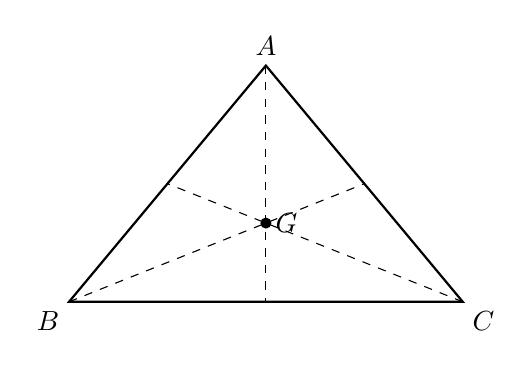
\begin{tikzpicture}
\coordinate (A) at (0,3);
\coordinate (B) at (-2.5,0);
\coordinate (C) at (2.5,0);
\coordinate (M) at (0,0);
\coordinate (N) at (1.25,1.5);
\coordinate (P) at (-1.25,1.5);

\draw[thick] (A)--(B)--(C)--cycle;
\draw[dashed] (A)--(M);
\draw[dashed] (B)--(N);
\draw[dashed] (C)--(P);

\fill (0,1) circle (2pt);
\node[right] at (0,1) {\(G\)};
\node[above] at (A) {\(A\)};
\node[below left] at (B) {\(B\)};
\node[below right] at (C) {\(C\)};
\end{tikzpicture}
\end{centereddiagram}

The point \(G\) is the centroid.

%%%%%%%%%%%%%%%%%%%%%%%%%%%%%%%%%%%%%%%%%%%%%%%%%%%%%%%%%%%%
\subsection{Perpendicular Bisectors and Circumcenter}
\label{subsec:circumcenter}
%%%%%%%%%%%%%%%%%%%%%%%%%%%%%%%%%%%%%%%%%%%%%%%%%%%%%%%%%%%%

A perpendicular bisector passes through the midpoint of a side at a right
angle.

The three perpendicular bisectors of a triangle meet at the
\emph{circumcenter}.

The circumcenter is equidistant from all three vertices.

Therefore it is the center of the triangle's circumscribed circle.

%%%%%%%%%%%%%%%%%%%%%%%%%%%%%%%%%%%%%%%%%%%%%%%%%%%%%%%%%%%%
\subsection{Angle Bisectors and Incenter}
\label{subsec:incenter}
%%%%%%%%%%%%%%%%%%%%%%%%%%%%%%%%%%%%%%%%%%%%%%%%%%%%%%%%%%%%

The three internal angle bisectors meet at the \emph{incenter}.

The incenter is equidistant from all three sides.

Therefore it is the center of the triangle's inscribed circle.

%%%%%%%%%%%%%%%%%%%%%%%%%%%%%%%%%%%%%%%%%%%%%%%%%%%%%%%%%%%%
\subsection{Altitudes and Orthocenter}
\label{subsec:orthocenter}
%%%%%%%%%%%%%%%%%%%%%%%%%%%%%%%%%%%%%%%%%%%%%%%%%%%%%%%%%%%%

\begin{definitionbox}{Altitude}
An \emph{altitude} of a triangle is a perpendicular segment from a vertex
to the line containing the opposite side.
\end{definitionbox}

The three altitude lines intersect at the \emph{orthocenter}.

Depending on the triangle, the orthocenter may lie:

\begin{itemize}
    \item inside an acute triangle;
    \item at the right-angle vertex of a right triangle;
    \item outside an obtuse triangle.
\end{itemize}

%%%%%%%%%%%%%%%%%%%%%%%%%%%%%%%%%%%%%%%%%%%%%%%%%%%%%%%%%%%%
\subsection{Triangle Centers Summary}
\label{subsec:triangle-centers-summary}
%%%%%%%%%%%%%%%%%%%%%%%%%%%%%%%%%%%%%%%%%%%%%%%%%%%%%%%%%%%%

\[
\begin{array}{c|c|c}
\textbf{Center} & \textbf{Intersection of} & \textbf{Key property}\\
\hline
\text{centroid} & \text{medians} & 2:1\text{ median ratio}\\
\text{circumcenter} & \text{perpendicular bisectors} & \text{equidistant from vertices}\\
\text{incenter} & \text{angle bisectors} & \text{equidistant from sides}\\
\text{orthocenter} & \text{altitudes} & \text{altitude intersection}
\end{array}
\]

%%%%%%%%%%%%%%%%%%%%%%%%%%%%%%%%%%%%%%%%%%%%%%%%%%%%%%%%%%%%
\subsection{Polygons}
\label{subsec:euclidean-polygons}
%%%%%%%%%%%%%%%%%%%%%%%%%%%%%%%%%%%%%%%%%%%%%%%%%%%%%%%%%%%%

\begin{definitionbox}{Polygon}
A \emph{polygon} is a closed plane figure formed by finitely many line
segments joined endpoint to endpoint.
\end{definitionbox}

Common polygons include:

\[
\begin{array}{c|c}
\textbf{Number of sides} & \textbf{Name}\\
\hline
3 & \text{triangle}\\
4 & \text{quadrilateral}\\
5 & \text{pentagon}\\
6 & \text{hexagon}\\
7 & \text{heptagon}\\
8 & \text{octagon}\\
9 & \text{nonagon}\\
10 & \text{decagon}
\end{array}
\]

%%%%%%%%%%%%%%%%%%%%%%%%%%%%%%%%%%%%%%%%%%%%%%%%%%%%%%%%%%%%
\subsection{Regular Polygons}
\label{subsec:regular-polygons}
%%%%%%%%%%%%%%%%%%%%%%%%%%%%%%%%%%%%%%%%%%%%%%%%%%%%%%%%%%%%

\begin{definitionbox}{Regular Polygon}
A polygon is \emph{regular} if all its sides are congruent and all its
interior angles are congruent.
\end{definitionbox}

Examples include equilateral triangles and squares.

%%%%%%%%%%%%%%%%%%%%%%%%%%%%%%%%%%%%%%%%%%%%%%%%%%%%%%%%%%%%
\subsection{Interior Angle Sum of a Polygon}
\label{subsec:polygon-interior-angle-sum}
%%%%%%%%%%%%%%%%%%%%%%%%%%%%%%%%%%%%%%%%%%%%%%%%%%%%%%%%%%%%

An \(n\)-sided polygon can be divided into

\[ n-2 \]

triangles.

Since each triangle contributes \(180^\circ\),

\begin{theorem}[Polygon Interior Angle Sum]
The sum of the interior angles of an \(n\)-gon is

\[ \boxed{(n-2)180^\circ.} \]
\end{theorem}

%%%%%%%%%%%%%%%%%%%%%%%%%%%%%%%%%%%%%%%%%%%%%%%%%%%%%%%%%%%%
\subsection{Worked Example: Polygon Angle Sum}
\label{subsec:worked-polygon-angle-sum}
%%%%%%%%%%%%%%%%%%%%%%%%%%%%%%%%%%%%%%%%%%%%%%%%%%%%%%%%%%%%

\begin{workedexamplebox}{Interior Angle Sum of an Octagon}

An octagon has

\[ n=8 \]

sides.

\begin{tabularx}{\textwidth}{@{}>{\raggedright\arraybackslash}p{0.43\textwidth}X@{}}
Use the polygon formula. & \((n-2)180^\circ\)\\
Substitute \(n=8\). & \((8-2)180^\circ\)\\
Simplify. & \(6(180^\circ)=1080^\circ\)
\end{tabularx}

\begin{answerbox}
\[ \boxed{1080^\circ} \]
\end{answerbox}
\end{workedexamplebox}

%%%%%%%%%%%%%%%%%%%%%%%%%%%%%%%%%%%%%%%%%%%%%%%%%%%%%%%%%%%%
\subsection{Interior Angles of Regular Polygons}
\label{subsec:regular-polygon-interior-angle}
%%%%%%%%%%%%%%%%%%%%%%%%%%%%%%%%%%%%%%%%%%%%%%%%%%%%%%%%%%%%

For a regular \(n\)-gon, all interior angles have equal measure.

Therefore each interior angle is

\[ \boxed{\frac{(n-2)180^\circ}{n}.} \]

%%%%%%%%%%%%%%%%%%%%%%%%%%%%%%%%%%%%%%%%%%%%%%%%%%%%%%%%%%%%
\subsection{Exterior Angles of Polygons}
\label{subsec:polygon-exterior-angles}
%%%%%%%%%%%%%%%%%%%%%%%%%%%%%%%%%%%%%%%%%%%%%%%%%%%%%%%%%%%%

Taking one exterior angle at each vertex of a convex polygon produces a full
rotation.

Therefore

\begin{theorem}[Exterior Angle Sum]
The exterior angles of a convex polygon sum to

\[ \boxed{360^\circ.} \]
\end{theorem}

For a regular \(n\)-gon, each exterior angle is

\[ \boxed{\frac{360^\circ}{n}.} \]

%%%%%%%%%%%%%%%%%%%%%%%%%%%%%%%%%%%%%%%%%%%%%%%%%%%%%%%%%%%%
\subsection{Quadrilaterals}
\label{subsec:euclidean-quadrilaterals}
%%%%%%%%%%%%%%%%%%%%%%%%%%%%%%%%%%%%%%%%%%%%%%%%%%%%%%%%%%%%

A quadrilateral has four sides.

Its interior angle sum is

\[ (4-2)180^\circ=360^\circ. \]

Important families include:

\begin{itemize}
    \item parallelograms;
    \item rectangles;
    \item rhombi;
    \item squares;
    \item trapezoids;
    \item kites.
\end{itemize}

%%%%%%%%%%%%%%%%%%%%%%%%%%%%%%%%%%%%%%%%%%%%%%%%%%%%%%%%%%%%
\subsection{Parallelograms}
\label{subsec:parallelograms}
%%%%%%%%%%%%%%%%%%%%%%%%%%%%%%%%%%%%%%%%%%%%%%%%%%%%%%%%%%%%

\begin{definitionbox}{Parallelogram}
A \emph{parallelogram} is a quadrilateral whose two pairs of opposite sides
are parallel.
\end{definitionbox}

Important properties include:

\begin{itemize}
    \item opposite sides are congruent;
    \item opposite angles are congruent;
    \item consecutive angles are supplementary;
    \item diagonals bisect each other.
\end{itemize}

%%%%%%%%%%%%%%%%%%%%%%%%%%%%%%%%%%%%%%%%%%%%%%%%%%%%%%%%%%%%
\subsection{Rectangles}
\label{subsec:rectangles}
%%%%%%%%%%%%%%%%%%%%%%%%%%%%%%%%%%%%%%%%%%%%%%%%%%%%%%%%%%%%

A rectangle is a parallelogram with four right angles.

Therefore it inherits all parallelogram properties.

Additionally, its diagonals are congruent.

%%%%%%%%%%%%%%%%%%%%%%%%%%%%%%%%%%%%%%%%%%%%%%%%%%%%%%%%%%%%
\subsection{Rhombi}
\label{subsec:rhombi}
%%%%%%%%%%%%%%%%%%%%%%%%%%%%%%%%%%%%%%%%%%%%%%%%%%%%%%%%%%%%

A rhombus is a parallelogram with four congruent sides.

Its diagonals:

\begin{itemize}
    \item bisect each other;
    \item are perpendicular;
    \item bisect opposite angles.
\end{itemize}

%%%%%%%%%%%%%%%%%%%%%%%%%%%%%%%%%%%%%%%%%%%%%%%%%%%%%%%%%%%%
\subsection{Squares}
\label{subsec:squares-euclidean}
%%%%%%%%%%%%%%%%%%%%%%%%%%%%%%%%%%%%%%%%%%%%%%%%%%%%%%%%%%%%

A square is both a rectangle and a rhombus.

Therefore a square has:

\begin{itemize}
    \item four congruent sides;
    \item four right angles;
    \item opposite parallel sides;
    \item congruent diagonals;
    \item perpendicular diagonals;
    \item diagonals that bisect each other;
    \item diagonals that bisect opposite angles.
\end{itemize}

%%%%%%%%%%%%%%%%%%%%%%%%%%%%%%%%%%%%%%%%%%%%%%%%%%%%%%%%%%%%
\subsection{Quadrilateral Hierarchy}
\label{subsec:quadrilateral-hierarchy}
%%%%%%%%%%%%%%%%%%%%%%%%%%%%%%%%%%%%%%%%%%%%%%%%%%%%%%%%%%%%

Using inclusive definitions, the hierarchy can be visualized as follows.

\begin{centereddiagram}
\begin{tikzpicture}[
node distance=1.1cm and 1.5cm,
every node/.style={draw,rounded corners,align=center,inner sep=5pt}
]
\node (Q) {Quadrilateral};
\node[below=of Q] (P) {Parallelogram};
\node[below left=of P] (R) {Rectangle};
\node[below right=of P] (H) {Rhombus};
\node[below=of P,yshift=-1.7cm] (S) {Square};

\draw[-{Latex[length=2.2mm]}] (S)--(R);
\draw[-{Latex[length=2.2mm]}] (S)--(H);
\draw[-{Latex[length=2.2mm]}] (R)--(P);
\draw[-{Latex[length=2.2mm]}] (H)--(P);
\draw[-{Latex[length=2.2mm]}] (P)--(Q);
\end{tikzpicture}
\end{centereddiagram}

Thus every square is a rectangle and a rhombus, and every rectangle and
rhombus is a parallelogram.

%%%%%%%%%%%%%%%%%%%%%%%%%%%%%%%%%%%%%%%%%%%%%%%%%%%%%%%%%%%%
\subsection{Circles}
\label{subsec:euclidean-circles}
%%%%%%%%%%%%%%%%%%%%%%%%%%%%%%%%%%%%%%%%%%%%%%%%%%%%%%%%%%%%

\begin{definitionbox}{Circle}
A \emph{circle} is the set of all points in a plane at a fixed distance from
a fixed point.
\end{definitionbox}

The fixed point is the \emph{center}.

The fixed distance is the \emph{radius}.

%%%%%%%%%%%%%%%%%%%%%%%%%%%%%%%%%%%%%%%%%%%%%%%%%%%%%%%%%%%%
\subsection{Circle Terminology}
\label{subsec:circle-terminology}
%%%%%%%%%%%%%%%%%%%%%%%%%%%%%%%%%%%%%%%%%%%%%%%%%%%%%%%%%%%%

Important circle terminology includes:

\begin{itemize}
    \item \textbf{radius}: segment from center to circle;
    \item \textbf{diameter}: chord passing through the center;
    \item \textbf{chord}: segment with endpoints on the circle;
    \item \textbf{secant}: line intersecting the circle twice;
    \item \textbf{tangent}: line intersecting the circle once;
    \item \textbf{arc}: portion of the circle.
\end{itemize}

%%%%%%%%%%%%%%%%%%%%%%%%%%%%%%%%%%%%%%%%%%%%%%%%%%%%%%%%%%%%
\subsection{Circle Visual}
\label{subsec:circle-visual}
%%%%%%%%%%%%%%%%%%%%%%%%%%%%%%%%%%%%%%%%%%%%%%%%%%%%%%%%%%%%

\begin{centereddiagram}
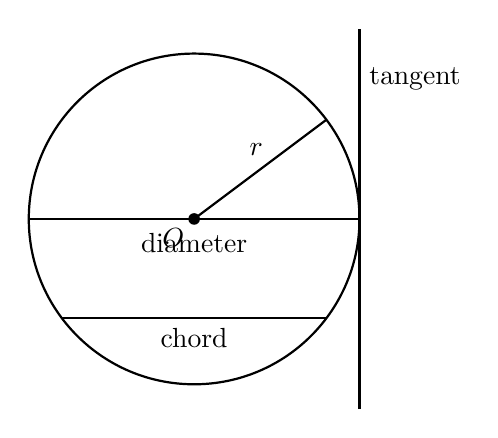
\begin{tikzpicture}[scale=1.05]
\draw[thick] (0,0) circle (2);
\fill (0,0) circle (2pt);
\node[below left] at (0,0) {\(O\)};

\draw[thick] (0,0)--(1.6,1.2);
\node[above] at (.75,.65) {\(r\)};

\draw[thick] (-2,0)--(2,0);
\node[below] at (0,-.05) {diameter};

\draw[thick] (-1.6,-1.2)--(1.6,-1.2);
\node[below] at (0,-1.2) {chord};

\draw[thick] (2,-2.3)--(2,2.3);
\node[right] at (2,1.7) {tangent};
\end{tikzpicture}
\end{centereddiagram}

%%%%%%%%%%%%%%%%%%%%%%%%%%%%%%%%%%%%%%%%%%%%%%%%%%%%%%%%%%%%
\subsection{Radius and Diameter}
\label{subsec:radius-diameter}
%%%%%%%%%%%%%%%%%%%%%%%%%%%%%%%%%%%%%%%%%%%%%%%%%%%%%%%%%%%%

If a circle has radius \(r\) and diameter \(d\), then

\[ \boxed{d=2r.} \]

Every diameter is a chord, but not every chord is a diameter.

The diameter is the longest possible chord of a circle.

%%%%%%%%%%%%%%%%%%%%%%%%%%%%%%%%%%%%%%%%%%%%%%%%%%%%%%%%%%%%
\subsection{Circumference}
\label{subsec:circumference-circle}
%%%%%%%%%%%%%%%%%%%%%%%%%%%%%%%%%%%%%%%%%%%%%%%%%%%%%%%%%%%%

The circumference of a circle is

\[ \boxed{C=2\pi r=\pi d.} \]

Here \(\pi\) is the circle constant, approximately

\[ \pi\approx3.14159265. \]

Its transcendence was discussed in
\cref{sec:transcendental-number-theory}.

%%%%%%%%%%%%%%%%%%%%%%%%%%%%%%%%%%%%%%%%%%%%%%%%%%%%%%%%%%%%
\subsection{Area of a Circle}
\label{subsec:circle-area}
%%%%%%%%%%%%%%%%%%%%%%%%%%%%%%%%%%%%%%%%%%%%%%%%%%%%%%%%%%%%

The area enclosed by a circle of radius \(r\) is

\[ \boxed{A=\pi r^2.} \]

The area grows quadratically with radius.

For example, doubling the radius multiplies the area by

\[ 2^2=4. \]

%%%%%%%%%%%%%%%%%%%%%%%%%%%%%%%%%%%%%%%%%%%%%%%%%%%%%%%%%%%%
\subsection{Central Angles}
\label{subsec:central-angles}
%%%%%%%%%%%%%%%%%%%%%%%%%%%%%%%%%%%%%%%%%%%%%%%%%%%%%%%%%%%%

A central angle has its vertex at the center of a circle.

The measure of a minor arc equals the measure of its corresponding central
angle.

Thus if

\[ m\angle AOB=80^\circ, \]

then the intercepted minor arc \(AB\) also has measure

\[ 80^\circ. \]

%%%%%%%%%%%%%%%%%%%%%%%%%%%%%%%%%%%%%%%%%%%%%%%%%%%%%%%%%%%%
\subsection{Inscribed Angles}
\label{subsec:inscribed-angles}
%%%%%%%%%%%%%%%%%%%%%%%%%%%%%%%%%%%%%%%%%%%%%%%%%%%%%%%%%%%%

An inscribed angle has its vertex on the circle.

\begin{theorem}[Inscribed Angle Theorem]
The measure of an inscribed angle equals half the measure of its intercepted
arc.
\end{theorem}

Thus

\[ \boxed{m\angle ABC=\frac12m\widehat{AC}.} \]

The notation

\[ \widehat{AC} \]

denotes arc \(AC\).

%%%%%%%%%%%%%%%%%%%%%%%%%%%%%%%%%%%%%%%%%%%%%%%%%%%%%%%%%%%%
\subsection{Angle in a Semicircle}
\label{subsec:angle-semicircle}
%%%%%%%%%%%%%%%%%%%%%%%%%%%%%%%%%%%%%%%%%%%%%%%%%%%%%%%%%%%%

A diameter intercepts a semicircle of measure

\[ 180^\circ. \]

Therefore an inscribed angle intercepting a diameter has measure

\[ \frac12(180^\circ)=90^\circ. \]

Hence:

\begin{theorem}[Thales' Theorem]
An angle inscribed in a semicircle is a right angle.
\end{theorem}

%%%%%%%%%%%%%%%%%%%%%%%%%%%%%%%%%%%%%%%%%%%%%%%%%%%%%%%%%%%%
\subsection{Tangent and Radius}
\label{subsec:tangent-radius}
%%%%%%%%%%%%%%%%%%%%%%%%%%%%%%%%%%%%%%%%%%%%%%%%%%%%%%%%%%%%

A tangent line is perpendicular to the radius drawn to the point of
tangency.

Thus if line \(\ell\) is tangent to a circle at \(P\) and \(O\) is the
center, then

\[ \boxed{OP\perp\ell.} \]

%%%%%%%%%%%%%%%%%%%%%%%%%%%%%%%%%%%%%%%%%%%%%%%%%%%%%%%%%%%%
\subsection{Perimeter}
\label{subsec:perimeter}
%%%%%%%%%%%%%%%%%%%%%%%%%%%%%%%%%%%%%%%%%%%%%%%%%%%%%%%%%%%%

The perimeter of a polygon is the sum of its side lengths.

For side lengths

\[ s_1,s_2,\ldots,s_n, \]

the perimeter is

\[ \boxed{P=s_1+s_2+\cdots+s_n.} \]

For a regular \(n\)-gon with side length \(s\),

\[ \boxed{P=ns.} \]

%%%%%%%%%%%%%%%%%%%%%%%%%%%%%%%%%%%%%%%%%%%%%%%%%%%%%%%%%%%%
\subsection{Area of Rectangles and Parallelograms}
\label{subsec:rectangle-parallelogram-area}
%%%%%%%%%%%%%%%%%%%%%%%%%%%%%%%%%%%%%%%%%%%%%%%%%%%%%%%%%%%%

For a rectangle,

\[ \boxed{A=bh.} \]

The same formula holds for a parallelogram:

\[ \boxed{A=bh,} \]

where \(h\) is the perpendicular height rather than the slanted side length.

%%%%%%%%%%%%%%%%%%%%%%%%%%%%%%%%%%%%%%%%%%%%%%%%%%%%%%%%%%%%
\subsection{Area of a Triangle}
\label{subsec:triangle-area}
%%%%%%%%%%%%%%%%%%%%%%%%%%%%%%%%%%%%%%%%%%%%%%%%%%%%%%%%%%%%

A triangle with base \(b\) and corresponding height \(h\) has area

\[ \boxed{A=\frac12bh.} \]

This follows by pairing the triangle with a congruent copy to form a
parallelogram of area \(bh\).

%%%%%%%%%%%%%%%%%%%%%%%%%%%%%%%%%%%%%%%%%%%%%%%%%%%%%%%%%%%%
\subsection{Triangle Area Visual}
\label{subsec:triangle-area-visual}
%%%%%%%%%%%%%%%%%%%%%%%%%%%%%%%%%%%%%%%%%%%%%%%%%%%%%%%%%%%%

\begin{centereddiagram}
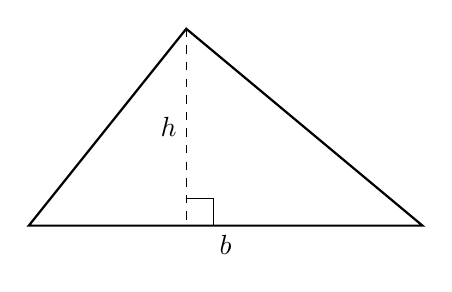
\begin{tikzpicture}
\coordinate (A) at (0,2.5);
\coordinate (B) at (-2,0);
\coordinate (C) at (3,0);
\coordinate (H) at (0,0);

\draw[thick] (A)--(B)--(C)--cycle;
\draw[dashed] (A)--(H);
\draw (0,0.35)--(0.35,0.35)--(0.35,0);

\node[left] at (0,1.25) {\(h\)};
\node[below] at (.5,0) {\(b\)};
\end{tikzpicture}
\end{centereddiagram}

%%%%%%%%%%%%%%%%%%%%%%%%%%%%%%%%%%%%%%%%%%%%%%%%%%%%%%%%%%%%
\subsection{Area of a Trapezoid}
\label{subsec:trapezoid-area}
%%%%%%%%%%%%%%%%%%%%%%%%%%%%%%%%%%%%%%%%%%%%%%%%%%%%%%%%%%%%

For parallel bases \(b_1,b_2\) and height \(h\),

\[ \boxed{A=\frac12(b_1+b_2)h.} \]

The quantity

\[ \frac{b_1+b_2}{2} \]

is the average of the two base lengths.

%%%%%%%%%%%%%%%%%%%%%%%%%%%%%%%%%%%%%%%%%%%%%%%%%%%%%%%%%%%%
\subsection{Area of a Rhombus or Kite}
\label{subsec:rhombus-kite-area}
%%%%%%%%%%%%%%%%%%%%%%%%%%%%%%%%%%%%%%%%%%%%%%%%%%%%%%%%%%%%

If the perpendicular diagonals have lengths \(d_1,d_2\), then

\[ \boxed{A=\frac12d_1d_2.} \]

%%%%%%%%%%%%%%%%%%%%%%%%%%%%%%%%%%%%%%%%%%%%%%%%%%%%%%%%%%%%
\subsection{Area of a Regular Polygon}
\label{subsec:regular-polygon-area}
%%%%%%%%%%%%%%%%%%%%%%%%%%%%%%%%%%%%%%%%%%%%%%%%%%%%%%%%%%%%

A regular polygon can be divided into congruent triangles by connecting its
center to each vertex.

If \(P\) is its perimeter and \(a\) is its apothem, then

\[ \boxed{A=\frac12aP.} \]

An \emph{apothem} is the perpendicular distance from the center of a regular
polygon to one of its sides.

%%%%%%%%%%%%%%%%%%%%%%%%%%%%%%%%%%%%%%%%%%%%%%%%%%%%%%%%%%%%
\subsection{Similarity and Area}
\label{subsec:similarity-area}
%%%%%%%%%%%%%%%%%%%%%%%%%%%%%%%%%%%%%%%%%%%%%%%%%%%%%%%%%%%%

Suppose two similar figures have corresponding lengths in ratio

\[ k. \]

Then their perimeters are in ratio

\[ k, \]

while their areas are in ratio

\[ \boxed{k^2.} \]

In three dimensions, corresponding volumes scale by

\[ k^3. \]

This distinction becomes increasingly important in geometry and modeling.

%%%%%%%%%%%%%%%%%%%%%%%%%%%%%%%%%%%%%%%%%%%%%%%%%%%%%%%%%%%%
\subsection{Worked Example: Similar Areas}
\label{subsec:worked-similar-areas}
%%%%%%%%%%%%%%%%%%%%%%%%%%%%%%%%%%%%%%%%%%%%%%%%%%%%%%%%%%%%

\begin{workedexamplebox}{Scaling Area}

Two similar triangles have corresponding side lengths in the ratio

\[ 3:5. \]

Find the ratio of their areas.

\begin{tabularx}{\textwidth}{@{}>{\raggedright\arraybackslash}p{0.43\textwidth}X@{}}
Use the length ratio. & \(\frac35\)\\
Square the ratio. & \(\left(\frac35\right)^2=\frac9{25}\)
\end{tabularx}

\begin{answerbox}
\[ \boxed{9:25} \]
\end{answerbox}
\end{workedexamplebox}

%%%%%%%%%%%%%%%%%%%%%%%%%%%%%%%%%%%%%%%%%%%%%%%%%%%%%%%%%%%%
\subsection{Rigid Motions}
\label{subsec:rigid-motions-euclidean}
%%%%%%%%%%%%%%%%%%%%%%%%%%%%%%%%%%%%%%%%%%%%%%%%%%%%%%%%%%%%

A \emph{rigid motion} preserves distances and angle measures.

The principal rigid motions of the Euclidean plane are:

\begin{itemize}
    \item translations;
    \item rotations;
    \item reflections;
    \item compositions of these transformations.
\end{itemize}

Rigid motions preserve congruence.

Transformation geometry is developed further in later geometric sections.

%%%%%%%%%%%%%%%%%%%%%%%%%%%%%%%%%%%%%%%%%%%%%%%%%%%%%%%%%%%%
\subsection{Translations}
\label{subsec:euclidean-translations}
%%%%%%%%%%%%%%%%%%%%%%%%%%%%%%%%%%%%%%%%%%%%%%%%%%%%%%%%%%%%

A translation moves every point the same distance in the same direction.

Schematically,

\[ P\longmapsto P'. \]

Distances, angles, parallelism, and orientation are preserved.

%%%%%%%%%%%%%%%%%%%%%%%%%%%%%%%%%%%%%%%%%%%%%%%%%%%%%%%%%%%%
\subsection{Rotations}
\label{subsec:euclidean-rotations}
%%%%%%%%%%%%%%%%%%%%%%%%%%%%%%%%%%%%%%%%%%%%%%%%%%%%%%%%%%%%

A rotation turns the plane about a fixed center through a fixed angle.

Every point moves along a circle centered at the rotation center.

Rotations preserve:

\begin{itemize}
    \item distance;
    \item angle measure;
    \item orientation.
\end{itemize}

%%%%%%%%%%%%%%%%%%%%%%%%%%%%%%%%%%%%%%%%%%%%%%%%%%%%%%%%%%%%
\subsection{Reflections}
\label{subsec:euclidean-reflections}
%%%%%%%%%%%%%%%%%%%%%%%%%%%%%%%%%%%%%%%%%%%%%%%%%%%%%%%%%%%%

A reflection flips the plane across a line called the \emph{line of
reflection}.

The line of reflection is the perpendicular bisector of the segment joining
a point to its image.

Reflections preserve distance and angle measure but reverse orientation.

%%%%%%%%%%%%%%%%%%%%%%%%%%%%%%%%%%%%%%%%%%%%%%%%%%%%%%%%%%%%
\subsection{Symmetry}
\label{subsec:euclidean-symmetry}
%%%%%%%%%%%%%%%%%%%%%%%%%%%%%%%%%%%%%%%%%%%%%%%%%%%%%%%%%%%%

A figure has a symmetry when some transformation maps the figure onto itself.

Common forms include:

\begin{itemize}
    \item reflectional symmetry;
    \item rotational symmetry.
\end{itemize}

For example, a square has four reflection axes and rotational symmetry
through multiples of

\[ 90^\circ. \]

Symmetry later becomes a central algebraic concept through group theory.

%%%%%%%%%%%%%%%%%%%%%%%%%%%%%%%%%%%%%%%%%%%%%%%%%%%%%%%%%%%%
\subsection{Straightedge and Compass Constructions}
\label{subsec:straightedge-compass}
%%%%%%%%%%%%%%%%%%%%%%%%%%%%%%%%%%%%%%%%%%%%%%%%%%%%%%%%%%%%

Classical Euclidean constructions permit two idealized tools:

\begin{itemize}
    \item an unmarked straightedge;
    \item a compass.
\end{itemize}

The straightedge constructs lines through known points.

The compass constructs circles with known centers and radii.

Together they can perform many exact geometric constructions.

%%%%%%%%%%%%%%%%%%%%%%%%%%%%%%%%%%%%%%%%%%%%%%%%%%%%%%%%%%%%
\subsection{Constructing a Perpendicular Bisector}
\label{subsec:construct-perpendicular-bisector}
%%%%%%%%%%%%%%%%%%%%%%%%%%%%%%%%%%%%%%%%%%%%%%%%%%%%%%%%%%%%

To construct the perpendicular bisector of \(\overline{AB}\):

\begin{enumerate}
    \item Draw circles of equal radius centered at \(A\) and \(B\).
    \item Choose the radius larger than \(\frac12AB\).
    \item Let the circles intersect at \(P\) and \(Q\).
    \item Draw \(\overleftrightarrow{PQ}\).
\end{enumerate}

The line \(\overleftrightarrow{PQ}\) is the perpendicular bisector of
\(\overline{AB}\).

%%%%%%%%%%%%%%%%%%%%%%%%%%%%%%%%%%%%%%%%%%%%%%%%%%%%%%%%%%%%
\subsection{Perpendicular Bisector Construction Visual}
\label{subsec:perpendicular-bisector-construction-visual}
%%%%%%%%%%%%%%%%%%%%%%%%%%%%%%%%%%%%%%%%%%%%%%%%%%%%%%%%%%%%

\begin{centereddiagram}
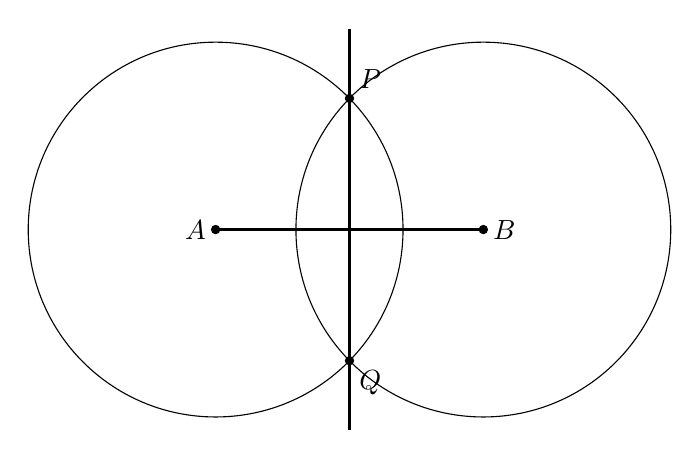
\begin{tikzpicture}[scale=0.85]
\coordinate (A) at (-2,0);
\coordinate (B) at (2,0);

\draw[thick] (A)--(B);
\draw (A) circle (2.8);
\draw (B) circle (2.8);

\coordinate (P) at (0,1.96);
\coordinate (Q) at (0,-1.96);

\draw[thick] (0,-3)--(0,3);

\fill (A) circle (2pt);
\fill (B) circle (2pt);
\fill (P) circle (2pt);
\fill (Q) circle (2pt);

\node[left] at (A) {\(A\)};
\node[right] at (B) {\(B\)};
\node[above right] at (P) {\(P\)};
\node[below right] at (Q) {\(Q\)};
\end{tikzpicture}
\end{centereddiagram}

%%%%%%%%%%%%%%%%%%%%%%%%%%%%%%%%%%%%%%%%%%%%%%%%%%%%%%%%%%%%
\subsection{Constructing an Angle Bisector}
\label{subsec:construct-angle-bisector}
%%%%%%%%%%%%%%%%%%%%%%%%%%%%%%%%%%%%%%%%%%%%%%%%%%%%%%%%%%%%

To bisect an angle:

\begin{enumerate}
    \item Draw an arc centered at the vertex intersecting both rays.
    \item From those two intersection points, draw arcs of equal radius.
    \item Mark their intersection inside the angle.
    \item Draw a ray from the original vertex through that intersection.
\end{enumerate}

The resulting ray divides the angle into two congruent angles.

%%%%%%%%%%%%%%%%%%%%%%%%%%%%%%%%%%%%%%%%%%%%%%%%%%%%%%%%%%%%
\subsection{Constructible Numbers}
\label{subsec:constructible-numbers-euclidean}
%%%%%%%%%%%%%%%%%%%%%%%%%%%%%%%%%%%%%%%%%%%%%%%%%%%%%%%%%%%%

Straightedge-and-compass constructions correspond algebraically to numbers
obtainable from rational numbers through a finite sequence of field
operations and square roots.

Consequently, constructible lengths are algebraic.

Not every algebraic number is constructible.

This algebraic viewpoint explains the impossibility of several classical
construction problems.

%%%%%%%%%%%%%%%%%%%%%%%%%%%%%%%%%%%%%%%%%%%%%%%%%%%%%%%%%%%%
\subsection{Classical Impossible Constructions}
\label{subsec:classical-impossible-constructions-geometry}
%%%%%%%%%%%%%%%%%%%%%%%%%%%%%%%%%%%%%%%%%%%%%%%%%%%%%%%%%%%%

Three famous problems are:

\begin{itemize}
    \item doubling the cube;
    \item trisecting an arbitrary angle;
    \item squaring the circle.
\end{itemize}

The first requires constructing

\[ \sqrt[3]{2}, \]

which is not straightedge-and-compass constructible.

General angle trisection leads to cubic equations that need not be
constructible.

Squaring the circle requires constructing

\[ \sqrt{\pi}. \]

Since \(\pi\) is transcendental, this is impossible.

%%%%%%%%%%%%%%%%%%%%%%%%%%%%%%%%%%%%%%%%%%%%%%%%%%%%%%%%%%%%
\subsection{Axioms, Definitions, and Theorems}
\label{subsec:geometry-axioms-definitions-theorems}
%%%%%%%%%%%%%%%%%%%%%%%%%%%%%%%%%%%%%%%%%%%%%%%%%%%%%%%%%%%%

Euclidean geometry is a deductive mathematical system.

Its logical structure can be summarized as

\[
\boxed{
\text{undefined terms}
\longrightarrow
\text{axioms}
\longrightarrow
\text{definitions}
\longrightarrow
\text{theorems}.
}
\]

An \emph{axiom} is accepted as a starting assumption.

A \emph{definition} specifies the meaning of a mathematical term.

A \emph{theorem} is a statement proved logically from previously accepted
results.

%%%%%%%%%%%%%%%%%%%%%%%%%%%%%%%%%%%%%%%%%%%%%%%%%%%%%%%%%%%%
\subsection{Structure of a Geometric Proof}
\label{subsec:geometric-proof-structure}
%%%%%%%%%%%%%%%%%%%%%%%%%%%%%%%%%%%%%%%%%%%%%%%%%%%%%%%%%%%%

A geometric proof typically begins with:

\begin{itemize}
    \item given information;
    \item a statement to prove.
\end{itemize}

The proof then forms a chain of justified statements.

Each step should follow from:

\begin{itemize}
    \item a definition;
    \item an axiom;
    \item a previously established theorem;
    \item algebra;
    \item a logical inference.
\end{itemize}

%%%%%%%%%%%%%%%%%%%%%%%%%%%%%%%%%%%%%%%%%%%%%%%%%%%%%%%%%%%%
\subsection{Worked Proof: Vertical Angles}
\label{subsec:proof-vertical-angles}
%%%%%%%%%%%%%%%%%%%%%%%%%%%%%%%%%%%%%%%%%%%%%%%%%%%%%%%%%%%%

Suppose two lines intersect and form angles \(\angle1,\angle2,\angle3\),
where \(\angle1\) and \(\angle3\) are vertical.

Because \(\angle1\) and \(\angle2\) form a linear pair,

\[ m\angle1+m\angle2=180^\circ. \]

Likewise,

\[ m\angle2+m\angle3=180^\circ. \]

Therefore

\[ m\angle1+m\angle2=m\angle2+m\angle3. \]

Subtracting \(m\angle2\) from both sides gives

\[ m\angle1=m\angle3. \]

Hence

\[ \boxed{\angle1\cong\angle3.} \]

This proves the Vertical Angles Theorem.

%%%%%%%%%%%%%%%%%%%%%%%%%%%%%%%%%%%%%%%%%%%%%%%%%%%%%%%%%%%%
\subsection{Worked Proof: Isosceles Triangle}
\label{subsec:proof-isosceles-triangle}
%%%%%%%%%%%%%%%%%%%%%%%%%%%%%%%%%%%%%%%%%%%%%%%%%%%%%%%%%%%%

Suppose

\[ AB=AC \]

in \(\triangle ABC\).

Construct the angle bisector of \(\angle A\), meeting \(\overline{BC}\) at
\(D\).

Then:

\[ AB=AC \]

by hypothesis,

\[ AD=AD \]

by the reflexive property, and

\[ \angle BAD\cong\angle DAC \]

because \(AD\) bisects \(\angle A\).

Therefore

\[ \triangle ABD\cong\triangle ACD \]

by SAS.

By corresponding parts of congruent triangles,

\[ \boxed{\angle B\cong\angle C.} \]

%%%%%%%%%%%%%%%%%%%%%%%%%%%%%%%%%%%%%%%%%%%%%%%%%%%%%%%%%%%%
\subsection{Proof and Diagrams}
\label{subsec:proof-and-diagrams}
%%%%%%%%%%%%%%%%%%%%%%%%%%%%%%%%%%%%%%%%%%%%%%%%%%%%%%%%%%%%

A diagram is an important reasoning aid, but it is not itself a proof.

A drawing may appear to show that:

\begin{itemize}
    \item two angles are equal;
    \item two lines are perpendicular;
    \item a point is a midpoint;
    \item two segments have equal length.
\end{itemize}

None of these may be assumed unless given or logically established.

\begin{warningbox}
Never conclude a geometric relationship solely because it appears true in a
diagram.

Diagrams illustrate hypotheses and conclusions; proofs justify them.
\end{warningbox}

%%%%%%%%%%%%%%%%%%%%%%%%%%%%%%%%%%%%%%%%%%%%%%%%%%%%%%%%%%%%
\subsection{Common Errors}
\label{subsec:euclidean-geometry-common-errors}
%%%%%%%%%%%%%%%%%%%%%%%%%%%%%%%%%%%%%%%%%%%%%%%%%%%%%%%%%%%%

\subsubsection{Confusing a Segment with Its Length}

The notation

\[ \overline{AB} \]

represents a geometric segment.

The notation

\[ AB \]

usually represents its length.

%%%%%%%%%%%%%%%%%%%%%%%%%%%%%%%%%%%%%%%%%%%%%%%%%%%%%%%%%%%%
\subsubsection{Writing Angle Names in the Wrong Order}

In

\[ \angle ABC, \]

the middle letter \(B\) must be the vertex.

%%%%%%%%%%%%%%%%%%%%%%%%%%%%%%%%%%%%%%%%%%%%%%%%%%%%%%%%%%%%
\subsubsection{Assuming Parallelism from a Picture}

Lines that appear parallel in a diagram are not necessarily known to be
parallel.

%%%%%%%%%%%%%%%%%%%%%%%%%%%%%%%%%%%%%%%%%%%%%%%%%%%%%%%%%%%%
\subsubsection{Assuming Perpendicularity from a Picture}

A \(90^\circ\) relationship must be given, marked, or proved.

%%%%%%%%%%%%%%%%%%%%%%%%%%%%%%%%%%%%%%%%%%%%%%%%%%%%%%%%%%%%
\subsubsection{Confusing Congruence and Similarity}

Congruent figures have the same shape and size.

Similar figures have the same shape but may have different sizes.

%%%%%%%%%%%%%%%%%%%%%%%%%%%%%%%%%%%%%%%%%%%%%%%%%%%%%%%%%%%%
\subsubsection{Using SSA as Congruence}

SSA is generally ambiguous and is not a universal congruence criterion.

%%%%%%%%%%%%%%%%%%%%%%%%%%%%%%%%%%%%%%%%%%%%%%%%%%%%%%%%%%%%
\subsubsection{Forgetting Correspondence Order}

If

\[ \triangle ABC\cong\triangle DEF, \]

then

\[ A\leftrightarrow D,\qquad B\leftrightarrow E,\qquad C\leftrightarrow F. \]

Incorrect correspondence produces incorrect side and angle relationships.

%%%%%%%%%%%%%%%%%%%%%%%%%%%%%%%%%%%%%%%%%%%%%%%%%%%%%%%%%%%%
\subsubsection{Using the Slanted Side as Height}

Area formulas involving height require perpendicular distance.

For a parallelogram,

\[ A=bh \]

uses the perpendicular height, not necessarily a side length.

%%%%%%%%%%%%%%%%%%%%%%%%%%%%%%%%%%%%%%%%%%%%%%%%%%%%%%%%%%%%
\subsubsection{Forgetting the Point at Infinity in Other Contexts}

Classical Euclidean circles do not contain a projective point at infinity.
Do not import projective or elliptic-curve conventions into ordinary
Euclidean diagrams unless the setting explicitly requires them.

%%%%%%%%%%%%%%%%%%%%%%%%%%%%%%%%%%%%%%%%%%%%%%%%%%%%%%%%%%%%
\subsection{Applications and Connections}
\label{subsec:euclidean-geometry-applications}
%%%%%%%%%%%%%%%%%%%%%%%%%%%%%%%%%%%%%%%%%%%%%%%%%%%%%%%%%%%%

\begin{applicationbox}
\textbf{Analytic Geometry.}
Coordinates convert Euclidean figures into equations and allow distances,
angles, intersections, and loci to be computed algebraically.

\medskip

\textbf{Vector Geometry.}
Vectors provide algebraic descriptions of displacement, direction,
parallelism, perpendicularity, and geometric transformations.

\medskip

\textbf{Trigonometry.}
Right triangles and similar triangles lead naturally to the trigonometric
ratios and the study of periodic functions.

\medskip

\textbf{Linear Algebra.}
Rotations, reflections, projections, and other geometric transformations can
be represented by matrices.

\medskip

\textbf{Group Theory.}
The symmetries of geometric objects form groups.

\medskip

\textbf{Topology.}
Topology studies properties preserved under continuous deformation rather
than rigid Euclidean measurement.

\medskip

\textbf{Differential Geometry.}
Euclidean geometry provides the local model from which curved spaces,
surfaces, and manifolds are studied.

\medskip

\textbf{Non-Euclidean Geometry.}
Changing the parallel postulate produces hyperbolic and elliptic geometric
systems.

\medskip

\textbf{Computational Geometry.}
Algorithms solve geometric problems involving intersections, distances,
polygons, triangulations, and spatial data.

\medskip

\textbf{Engineering and Physics.}
Lengths, angles, areas, volumes, projections, and geometric constraints are
fundamental in design, mechanics, surveying, navigation, and modeling.
\end{applicationbox}

%%%%%%%%%%%%%%%%%%%%%%%%%%%%%%%%%%%%%%%%%%%%%%%%%%%%%%%%%%%%
\subsection{Exercises}
\label{subsec:euclidean-geometry-exercises}
%%%%%%%%%%%%%%%%%%%%%%%%%%%%%%%%%%%%%%%%%%%%%%%%%%%%%%%%%%%%

\begin{exercise}[1]
Explain the difference between

\[ \overleftrightarrow{AB},\qquad\overline{AB},\qquad\overrightarrow{AB}. \]
\end{exercise}

\begin{exercise}[1]
If \(B\) lies between \(A\) and \(C\), \(AB=9\), and \(BC=14\), find \(AC\).
\end{exercise}

\begin{exercise}[1]
If \(M\) is the midpoint of \(\overline{AB}\) and \(AB=26\), find \(AM\).
\end{exercise}

\begin{exercise}[1]
Classify an angle measuring \(37^\circ\).
\end{exercise}

\begin{exercise}[1]
Classify an angle measuring \(90^\circ\).
\end{exercise}

\begin{exercise}[1]
Classify an angle measuring \(143^\circ\).
\end{exercise}

\begin{exercise}[1]
Find the complement of \(38^\circ\).
\end{exercise}

\begin{exercise}[1]
Find the supplement of \(127^\circ\).
\end{exercise}

\begin{exercise}[2]
Two vertical angles have measures \(4x+7^\circ\) and \(7x-29^\circ\).
Find \(x\) and the angle measure.
\end{exercise}

\begin{exercise}[2]
Two angles form a linear pair. Their measures are \(3x+20^\circ\) and
\(5x-8^\circ\). Find \(x\).
\end{exercise}

\begin{exercise}[1]
State Euclid's parallel postulate in the point-line form used in this
section.
\end{exercise}

\begin{exercise}[2]
Explain the difference between corresponding angles and alternate interior
angles.
\end{exercise}

\begin{exercise}[2]
If parallel lines are cut by a transversal and one angle measures
\(64^\circ\), determine the possible measures of all angles formed.
\end{exercise}

\begin{exercise}[1]
Classify a triangle with side lengths \(5,5,8\).
\end{exercise}

\begin{exercise}[1]
Classify a triangle containing a \(90^\circ\) angle.
\end{exercise}

\begin{exercise}[1]
A triangle has angles \(35^\circ\) and \(72^\circ\). Find the third angle.
\end{exercise}

\begin{exercise}[2]
An exterior angle of a triangle measures \(128^\circ\). One remote interior
angle measures \(53^\circ\). Find the other remote interior angle.
\end{exercise}

\begin{exercise}[2]
Can lengths \(5,8,14\) form a triangle? Explain using the Triangle
Inequality.
\end{exercise}

\begin{exercise}[2]
Can lengths \(6,9,12\) form a triangle? Explain.
\end{exercise}

\begin{exercise}[2]
State the SSS, SAS, ASA, AAS, and HL triangle congruence criteria.
\end{exercise}

\begin{exercise}[2]
Explain why SSA is not generally sufficient to establish triangle
congruence.
\end{exercise}

\begin{exercise}[2]
Explain the meaning of CPCTC.
\end{exercise}

\begin{exercise}[1]
If

\[ \triangle ABC\sim\triangle DEF \]

and \(AB=8\), \(DE=12\), and \(BC=10\), find \(EF\).
\end{exercise}

\begin{exercise}[2]
Two similar figures have scale factor \(4\). What is their area scale
factor?
\end{exercise}

\begin{exercise}[2]
Two similar solids have scale factor \(3\). What is their volume scale
factor?
\end{exercise}

\begin{exercise}[1]
A right triangle has legs \(9\) and \(12\). Find its hypotenuse.
\end{exercise}

\begin{exercise}[1]
A right triangle has hypotenuse \(13\) and one leg \(5\). Find the other
leg.
\end{exercise}

\begin{exercise}[2]
Determine whether side lengths \(7,24,25\) form a right triangle.
\end{exercise}

\begin{exercise}[1]
Find the hypotenuse of a \(45^\circ-45^\circ-90^\circ\) triangle whose leg
has length \(7\).
\end{exercise}

\begin{exercise}[1]
The short leg of a \(30^\circ-60^\circ-90^\circ\) triangle has length \(6\).
Find the other two sides.
\end{exercise}

\begin{exercise}[1]
Name the intersection point of the three medians of a triangle.
\end{exercise}

\begin{exercise}[1]
Name the intersection point of the three perpendicular bisectors.
\end{exercise}

\begin{exercise}[1]
Name the intersection point of the three angle bisectors.
\end{exercise}

\begin{exercise}[1]
Name the intersection point of the three altitudes.
\end{exercise}

\begin{exercise}[2]
A median has total length \(15\). Find the distance from the vertex to the
centroid.
\end{exercise}

\begin{exercise}[1]
Find the interior angle sum of a decagon.
\end{exercise}

\begin{exercise}[1]
Find each interior angle of a regular hexagon.
\end{exercise}

\begin{exercise}[1]
Find each exterior angle of a regular nonagon.
\end{exercise}

\begin{exercise}[2]
How many sides does a regular polygon have if each exterior angle measures
\(24^\circ\)?
\end{exercise}

\begin{exercise}[2]
Explain why every square is a rectangle.
\end{exercise}

\begin{exercise}[2]
Explain why every square is a rhombus.
\end{exercise}

\begin{exercise}[2]
Is every rectangle a square? Explain.
\end{exercise}

\begin{exercise}[1]
A circle has radius \(8\). Find its diameter and circumference.
\end{exercise}

\begin{exercise}[1]
A circle has diameter \(14\). Find its radius and area.
\end{exercise}

\begin{exercise}[2]
An inscribed angle intercepts an arc measuring \(110^\circ\). Find the angle
measure.
\end{exercise}

\begin{exercise}[2]
An inscribed angle measures \(42^\circ\). Find the measure of its intercepted
arc.
\end{exercise}

\begin{exercise}[2]
Explain why an angle inscribed in a semicircle is a right angle.
\end{exercise}

\begin{exercise}[1]
Find the area of a triangle with base \(12\) and height \(9\).
\end{exercise}

\begin{exercise}[1]
Find the area of a parallelogram with base \(14\) and perpendicular height
\(6\).
\end{exercise}

\begin{exercise}[1]
Find the area of a trapezoid with bases \(8\) and \(14\) and height \(5\).
\end{exercise}

\begin{exercise}[2]
A regular polygon has perimeter \(48\) and apothem \(7\). Find its area.
\end{exercise}

\begin{exercise}[2]
Two similar triangles have corresponding side ratio \(2:7\). Find the ratio
of their areas.
\end{exercise}

\begin{exercise}[2]
Describe the difference between a translation, rotation, and reflection.
\end{exercise}

\begin{exercise}[2]
Which rigid motions preserve orientation?
\end{exercise}

\begin{exercise}[2]
Explain why a square has rotational symmetry of order \(4\).
\end{exercise}

\begin{exercise}[2]
Describe the straightedge-and-compass construction of a perpendicular
bisector.
\end{exercise}

\begin{exercise}[2]
Explain why constructible numbers must be algebraic.
\end{exercise}

\begin{exercise}[2]
Explain why the transcendence of \(\pi\) rules out squaring the circle.
\end{exercise}

\begin{exercise}[3]
Prove the Vertical Angles Theorem using linear pairs.
\end{exercise}

\begin{exercise}[3]
Prove the Isosceles Triangle Theorem using SAS congruence.
\end{exercise}

\begin{exercise}[3]
Prove that the interior angles of a quadrilateral sum to \(360^\circ\) by
dividing the quadrilateral into triangles.
\end{exercise}

\begin{exercise}[3]
Prove that the exterior angles of a convex polygon sum to \(360^\circ\).
\end{exercise}

\begin{exercise}[3]
Explain how the Euclidean parallel postulate is used in the standard proof
of the Triangle Sum Theorem.
\end{exercise}

\begin{exercise}[3]
Explain why diagrams alone cannot establish geometric facts.
\end{exercise}

%%%%%%%%%%%%%%%%%%%%%%%%%%%%%%%%%%%%%%%%%%%%%%%%%%%%%%%%%%%%
\subsection{Conceptual Summary}
\label{subsec:euclidean-geometry-summary}
%%%%%%%%%%%%%%%%%%%%%%%%%%%%%%%%%%%%%%%%%%%%%%%%%%%%%%%%%%%%

Euclidean geometry studies points, lines, planes, angles, figures, distance,
and spatial relationships in flat space.

Its basic objects include

\[
\boxed{
\text{points},\quad
\text{lines},\quad
\text{segments},\quad
\text{rays},\quad
\text{planes},\quad
\text{angles}.
}
\]

Segment and angle addition provide fundamental measurement relationships.

Parallel and perpendicular lines organize the geometry of the plane.

When parallel lines are intersected by a transversal, corresponding and
alternate angles become congruent while same-side interior angles become
supplementary.

Triangles form one of the central structures of Euclidean geometry.

Their angles satisfy

\[ \boxed{\alpha+\beta+\gamma=180^\circ.} \]

Congruence criteria such as

\[
\mathrm{SSS},\qquad
\mathrm{SAS},\qquad
\mathrm{ASA},\qquad
\mathrm{AAS},\qquad
\mathrm{HL}
\]

allow complete geometric equality to be established from limited
information.

Similarity preserves shape and produces proportional corresponding lengths.

For right triangles,

\[ \boxed{a^2+b^2=c^2.} \]

Medians, perpendicular bisectors, angle bisectors, and altitudes determine
the centroid, circumcenter, incenter, and orthocenter.

Polygon angle sums follow from decomposition into triangles:

\[ \boxed{S=(n-2)180^\circ.} \]

The exterior angles of a convex polygon satisfy

\[ \boxed{S_{\mathrm{ext}}=360^\circ.} \]

For circles,

\[ \boxed{C=2\pi r,\qquad A=\pi r^2.} \]

Area formulas arise from geometric decomposition and rearrangement.

Rigid motions preserve Euclidean distance and angle measure, providing a
transformation-based interpretation of congruence.

Straightedge-and-compass constructions connect classical geometry with
algebraic field extensions.

Finally, Euclidean geometry is fundamentally deductive:

\[
\boxed{
\text{axioms}
\longrightarrow
\text{definitions}
\longrightarrow
\text{theorems}
\longrightarrow
\text{proofs}.
}
\]

Its concepts provide the geometric foundation for analytic geometry, vector
geometry, trigonometry, differential geometry, topology, and many branches
of applied mathematics.

%%%%%%%%%%%%%%%%%%%%%%%%%%%%%%%%%%%%%%%%%%%%%%%%%%%%%%%%%%%%
\subsection{Section Connections}
\label{subsec:euclidean-geometry-connections}
%%%%%%%%%%%%%%%%%%%%%%%%%%%%%%%%%%%%%%%%%%%%%%%%%%%%%%%%%%%%

\chapterconnection{
Euclidean Geometry begins the Geometry chapter by establishing the classical
language of points, lines, angles, triangles, polygons, circles, congruence,
similarity, measurement, construction, and proof. Analytic Geometry will
introduce coordinates and translate these relationships into algebraic
equations. Vector Geometry will replace many synthetic relationships with
vector operations. Affine and Projective Geometry will identify which
Euclidean properties survive under broader transformations. Non-Euclidean
Geometry will investigate what changes when the Euclidean parallel postulate
is replaced. Differential Geometry will extend geometric reasoning to
curves, surfaces, manifolds, and curved spaces. Discrete and Computational
Geometry will study finite geometric structures and algorithms. Euclidean
geometry therefore serves as the classical foundation from which the later
geometric theories are developed.
}

%%%%%%%%%%%%%%%%%%%%%%%%%%%%%%%%%%%%%%%%%%%%%%%%%%%%%%%%%%%%
% SECTION SOURCE TRACKING
%%%%%%%%%%%%%%%%%%%%%%%%%%%%%%%%%%%%%%%%%%%%%%%%%%%%%%%%%%%%

%------------------------------------------------------------
% 3.1 Euclidean Geometry
%------------------------------------------------------------
%
% Source basis:
%   - Standard classical Euclidean geometry.
%
% Used for:
%   - points, lines, segments, rays, and planes;
%   - incidence and betweenness;
%   - segment and angle addition;
%   - congruent segments and angles;
%   - angle classification;
%   - complementary and supplementary angles;
%   - vertical angles and linear pairs;
%   - parallel and perpendicular lines;
%   - Euclidean parallel postulate;
%   - transversals and parallel-line angle relationships;
%   - triangle classification;
%   - Triangle Sum Theorem;
%   - exterior angles;
%   - Triangle Inequality;
%   - triangle congruence criteria;
%   - triangle similarity criteria;
%   - Pythagorean Theorem;
%   - special right triangles;
%   - triangle centers;
%   - polygons and quadrilaterals;
%   - polygon angle sums;
%   - circle terminology and elementary circle theorems;
%   - perimeter and area;
%   - rigid motions and symmetry;
%   - straightedge-and-compass constructions;
%   - constructibility;
%   - elementary synthetic proofs.
%
% Notes:
%   - Coordinate formulas and coordinate methods belong
%     canonically to Analytic / Coordinate Geometry.
%   - Vector methods belong canonically to Vector Geometry.
%   - Full transformation-group treatment belongs to later
%     geometry and algebra sections.
%   - The algebraic theory of constructible numbers connects
%     back to Field Theory and Galois Theory.
%   - Non-Euclidean alternatives to the parallel postulate
%     are developed canonically in Non-Euclidean Geometry.
%
%%%%%%%%%%%%%%%%%%%%%%%%%%%%%%%%%%%%%%%%%%%%%%%%%%%%%%%%%%%%